\documentclass{book}
\usepackage{graphicx}
\usepackage[english]{babel}
\usepackage{amsthm}
\usepackage{amssymb}
\usepackage{amsfonts}
\usepackage{mdframed}
\usepackage{physics}
\usepackage{tikz}
\usepackage[a4paper, margin=1in]{geometry}
\geometry{a4paper, margin=1in}
\usepackage{xcolor}
\usetikzlibrary{arrows.meta}
\usetikzlibrary{angles,quotes}
\graphicspath{ {./images/} }
\usepackage{svg}
\usepackage{subcaption}
\usepackage{bm}
\usepackage{empheq}
\usepackage{cancel}
\usetikzlibrary{decorations.text}
\usepackage[most]{tcolorbox}
\usepackage{tensor}
%3D
\usepackage{mathtools}
\usepackage{booktabs}
\usepackage{array}
\newcolumntype{C}{>{$}c<{$}}
\usepackage{tikz-3dplot}
\usepackage{appendix}
\usepackage{pgfplots}
\usetikzlibrary{shapes.geometric}
\usetikzlibrary{calc,patterns,angles,quotes}
%Tikz Library
\usetikzlibrary{angles, quotes, intersections}
\usepackage[bb=dsserif]{mathalpha}
\usetikzlibrary{decorations.pathmorphing}

\tikzset{snake it/.style={decorate, decoration=snake}}
\usetikzlibrary {patterns,patterns.meta} 
\usepackage{etoolbox} % ifthen
\usepackage[outline]{contour} % glow around text
\usetikzlibrary{calc} % for adding up coordinates
\usetikzlibrary{decorations.markings,decorations.pathmorphing}
\usetikzlibrary{angles,quotes} % for pic (angle labels)
\usetikzlibrary{arrows.meta} % for arrow size
\usepackage{xfp} % higher precision (16 digits?)

\usepackage{tcolorbox}

\def\innerproduct#1#2{{\langle #1},{#2 \rangle}}
\renewcommand{\braket}[2]{\langle#1|#2\rangle}

%https://osl.ugr.es/CTAN/macros/latex/contrib/tcolorbox/tcolorbox.pdf
\tcbuselibrary{breakable}
\tcbset{%any default parameters
	width=0.7\textwidth,
	halign=justify,
	center,
	breakable,
	colback=white    
}
\DeclareMathOperator{\mRe}{Re}
\DeclareMathOperator{\mIm}{Im}
\newenvironment{aside}
{\begin{mdframed}[style=0,%
		leftline=false,rightline=false,leftmargin=2em,rightmargin=2em,%
		innerleftmargin=0pt,innerrightmargin=0pt,linewidth=0.75pt,%
		skipabove=7pt,skipbelow=7pt]\small}
	{\end{mdframed}}

\renewcommand{\cleardoublepage}{\clearpage}

\title{Complex Variables and Vector Spaces}
\author{Dominik Szablonski}
\newtheorem{law}{Law}
\newtheorem{klaw}{Law}

\newtcbtheorem{Definitions}{Definition}%
{colback=blue!5!white,colframe=blue!75!black,width=\textwidth,fonttitle=\bfseries}{}

\newtcbtheorem{Theorems}{Theorem}%
{colback=red!5!white,colframe=red!75!black,width=\textwidth,fonttitle=\bfseries}{}

\newtcbtheorem{Examples}{Example}%
{colback=yellow!5!white,colframe=yellow!75!black,width=\textwidth,fonttitle=\bfseries}{}

\newtcbtheorem{Lemma}{Lemma}%
{colback=orange!5!white,colframe=orange!75!black,width=\textwidth,fonttitle=\bfseries}{}

\def\doubleunderline#1{\underline{\underline{#1}}}

\newtheorem*{theorem}{Theorem}
\newcommand*\circled[1]{\tikz[baseline=(char.base)]{
		\node[shape=circle,draw,minimum size=4mm, inner sep=0pt] (char)
		{\rule[-3pt]{0pt}{\dimexpr2ex+2pt}#1};}}

\setlength\parindent{0pt}
\pgfplotsset{compat=1.18}
\begin{document}
\maketitle

\tableofcontents

\chapter{Vector Spaces}
We wish to generalise the idea of a vector and field. Let us first define a field,
\begin{Definitions}{Fields}{}
	A field $\mathbb{F}$ is a set with 2 binary operations defined on it, addition $(+)$ and multiplication $(\cdot)$. The following axioms hold $\forall a,b,c \in \mathbb{F}$,
	\begin{enumerate}
		\item \textit{Associativity}, \begin{align}
			a + (b + c) = (a + b) + c &&
			a \cdot (b\cdot c) = (a\cdot b) \cdot c
		\end{align}
		\item \textit{Commutativity}, \begin{align}
			a + b = b + a &&
			a\cdot b = b\cdot a
		\end{align}
		\item \textit{Identity}. $\exists 0, 1 \in \mathbb{F}$ such that,
		\begin{align}
			a + 0 = a &&
			a\cdot 1 = a
		\end{align}
		\item \textit{Additive inverse.} $\forall a \in \mathbb{F}, \exists -a \in \mathbb{F}$ such that,
		\begin{equation}
			a + (-a) = 0.
		\end{equation}
		\item \textit{Multiplicative inverse.} $\forall a \in \mathbb{F}, \exists a^{-1} \in \mathbb{F}$ such that,
		\begin{equation}
			a \cdot a^{-1} = 1.
		\end{equation}
	\end{enumerate}
\end{Definitions}
We can then define a vector space,
\begin{Definitions}{Vector Space}{}
	Let $\mathbb{F}$ be a field. A vector space $V$ over $\mathbb{F}$ is a set of objects $\vb{u}, \vb{v}, \vb{w},\ldots$ which satisfy,
	\begin{enumerate}
		\item \textit{Addition.} The set is closed under addition, such that $\vb{u}, \vb{v} \in V \implies \vb{w} = \vb{u} + \vb{v} \in V$. This operation is commutative and associative.
		\item \textit{Scalar multiplication.} The set is closed under multiplication by a scalar, i.e., $\vb{u} \in V \implies \lambda \vb{u}\in V$ for $\lambda \in \mathbb{F}$. Scalar multiplication is associative and distributive.
		\item \textit{Null vector.} $\exists \vb{0}, \vb{u} + \vb{0} = \vb{u}$.
		\item \textit{Negative vector.} $\forall \vb{u} \in V, \exists -\vb{u} \in V$ such that,
		\begin{equation}
			\vb{u} + (-\vb{u}) = 0.
		\end{equation} 
	\end{enumerate}
\end{Definitions}
\section{Linear Independence}
If vectors are linearly independent, then they cannot be written as a combination of each other. Let us write down the formal definition,
\begin{Definitions}{Linear Independence}{}
	A set of vectors $\left\{\vb{u}_i \text{ for } i = 1, 2, \ldots, n\right\}$ is linearly independent if the equation,
	\begin{equation}
		\sum_j^n \lambda_j\vb{u}_j = \vb{0}
	\end{equation}
	has only 1 solution, $\forall i : \lambda_i = 0$.
\end{Definitions}
\section{Postulate of Dimensionality and Basis Vectors}
\begin{Definitions}{Dimensionality}{}
	A vector space $V$ has dimensions $N$ if it can accommodate no more than $N$ linearly independent vectors $\vb{u}_j$.
\end{Definitions}
We often denote $N$ dimensional vector spaces over a field $\mathbb{F}$ as $\mathbb{F}^N$, or more generally $V_N$. We are often also interested in the \textit{span} of a vector space.
\begin{Definitions}{Span}{}
	The span of a set of vectors $\left\{\vb{u}_i, for i=1,2,\ldots,n\right\}$ is the set of all vectors which can be written as a linear combination of $\vb{u}_i$.
\end{Definitions}
The above definition naturally leads to the below theorem,
\begin{Theorems}{}{}
	In an $N$-dimensional vector space $V_N$, any vector $\vb{u}$ can be written as a linear combination of $N$ linearly independent basis vectors $\vb{e}_j$.
\end{Theorems}
\begin{proof}
	Since there are no more than $N$ linearly independent vectors, the set of vectors $\left\{\vb{e}_i\right\}_{i=1}^{N} + \vb{u}$ must be linearly dependent. Therefore, there must be a relation of the form,
	\begin{equation}
		\sum_{i=1}^{N} \lambda_i\vb{e}_i + \lambda_0\vb{u} = \vb{0},
	\end{equation}
	where $\vb{u} \in V_N$ is an arbitrary vector and $\exists \lambda_i \neq 0$. From the definition of linear dependence, we require $\lambda_0 \vb{u}_0 \neq 0$, so,
	\begin{equation}
		\vb{u} = - \frac{1}{\lambda_0}\sum_{i=1}^{N}\lambda_i\vb{e}_i = \sum_i^Nu_i\vb{e}_i
	\end{equation}
	where $u_i = -\frac{\lambda_i}{\lambda_0}$.
\end{proof}
From the above theorem, we are able to define the \textbf{basis} of a vector space,
\begin{Definitions}{Basis}{}
	Any set of $N$ linearly independent vectors in $V_n$ is called a \textbf{basis}, and then \textbf{span} $V_N$, or synonymously, they are \textbf{complete} if $N$ is finite.
\end{Definitions}
This allows us to write any vector $\vb{v} \in V_N$ as,
\begin{equation}
	\vb{v} = \sum_i^Nv_i\vb{e}_i
\end{equation}
where $\vb{e}_i$ is any complete basis.
\section{Linear Subspaces}
We can consider a subspace of $V_N$ as a vector space spanned by a set of $M < N$ linearly independent vectors. The subspace $V_M$ must satisfy the following properties,
\begin{enumerate}
	\item It must contain the zero vector $\vb{0}$.
	\item It must be closed under addition and scalar multiplication.
\end{enumerate}
An example of a subspace would be the subspace of $\mathbb{R}^3$ which is the set of vectors $(x,y,0)$, where $x,y \in \mathbb{R}$ which define the $xy$-plane in $\mathbb{R}^3$. This is a case of a more general result,
\begin{Theorems}{Subspaces}{}
	Any set of $M$ $(M \leq N)$ linearly independent vectors $\left\{\vb{e}_i\right\}^M_{i=1}$ in $V_N$ span a subspace $V_M$ of $V_N$.
\end{Theorems}
However, counterexamples do exist such as the set of vectors lying within a unit circle $\left\{(x,y):x^2+y^2 \leq 1\right\}$ which cannot be a subspace of $\mathbb{R}^3$ This is because we can choose a $\lambda$ such that $\lambda x_1$ or $\lambda y_1 > 1$ lies outside of the unit circle, and thus is not closed under multiplication.
\section{Normed Spaces}
We wish to now generalise length in order to define the closeness of vectors. We do this by defining a \textit{norm}.
\begin{Definitions}{Norm}{}
	Give a vector space $V$ over a field $\mathbb{F}$, a norm on $V$ is a real-valued function $p : V \to \mathbb{R}$ with the following properties,
	\begin{enumerate}
		\item \textbf{Triangle Inequality}, $p(\mathbf{x} + \mathbf{y}) \leq p(\mathbf{x}) + p(\mathbf{y}), \forall \mathbf{x}, \mathbf{y} \in V$
		\item \textbf{Absolute Homogeneity}, $p(sx) = \abs{s}p(\vb{x}), \forall \mathbf{x} \in V, \forall s \in \mathbb{R}$.
		\item \textbf{Positive Definiteness}, $\forall \vb{x} \in V, p(x) \geq 0; p(x) = 0 \iff x = 0$.
	\end{enumerate}
\end{Definitions}
For a vector space $V_N$ and two vectors $\vb{u},\vb{v} \in V_N$, the distance between them is given by $\norm{\vb{u} - \vb{v}}$. There are different types of norms, some of which are defined in sections below. 
\subsection{Supremum Norm}
$\forall \vb{x} \in V_N$ where $x_i$ are the components in a given basis, the we define the \textit{supremum} or \textit{infinity} norm.
\begin{Definitions}{Supremum Norm}{}
	\begin{equation}
		\norm{\vb{x}}_S = \norm{\vb{x}}_{\infty} = \max_i\abs{x_i}.
	\end{equation}
\end{Definitions}
It can be shown that, since $\abs{a + b} \leq \abs{a} + \abs{b}$ $\forall a,b \in \mathbb{R}$ or $\forall a,b \in \mathbb{C}$,
\begin{equation}
	\begin{split}
		\norm{\vb{x} + {y}} = \max_i\abs{x_i + y_i} & \leq \max_i\left(\abs{x_i} + \abs{y_i}\right) \\
		& \leq \max_i\abs{x_i} + \max_j\abs{y}
	\end{split}
\end{equation}
\subsection{1-Norm}
$\forall \vb{x} \in V_N$ where $x_i$ are the components of $\vb{x}$, we define the 1-norm,
\begin{Definitions}{1-Norm}{}
	\begin{equation}
		\norm{x}_1 = \sum_{i=1}^N \abs{x_i}.
	\end{equation}
\end{Definitions}
\section{Completeness}
\subsection{Cauchy Sequences}
\begin{Definitions}{Cauchy Sequence}{}
	A sequence $\left\{a_n\right\}_{n=0}^{\infty}$, $a_n \in V$ and $V$ is a normed vector space is Cauchy if $\forall \epsilon > 0, \exists N > 0$ such that $\forall n,m > N, \norm{a_n - a_m} < \epsilon$.
\end{Definitions}{}{}
Let us consider some sequences and show if they are Cauchy.
\subsubsection{Sequences over $\mathbb{R}$}
	\begin{figure}
		\centering
	\begin{tikzpicture}
		\begin{axis}[%
			,axis x line = bottom,axis y line = left
			,ytick=\empty, xtick=\empty
			,ymax=5, xmax=3 % or enlarge y limits=upper
			]
			\addplot+[const plot, no marks, very thick, color=black] coordinates {(0,4) (0.5,1) (1,0.444) (1.5,0.25) (2,0.16) (2.5,0.111)};
			\addplot+[no marks, thick, dashed, color=red, domain=0:5,samples=100] plot {1/(\x*\x) };
			\node[anchor = west] at (0.5,4) {$\displaystyle\frac{1}{(m+1)^2}$};
			\node[anchor = south] at (2.5,0.111) {$\displaystyle\frac{1}{n^2}$};
			\node at (0.8, 2.5) {$\displaystyle\frac{1}{x^2}$};
		\end{axis}
	\end{tikzpicture}
	\caption{Graphical proof used in example 1.}
	\label{fig:proof1}
\end{figure}
\begin{Examples}{$a_n = \sum_{i=1} \frac{1}{i^2}$}{}
	A sequence in $\mathbb{R}$ with $\norm{a} = \abs{a}$ is
	\begin{equation}
		a_n =  \sum_{i=1}^{n}\frac{1}{i^2}.
	\end{equation}
	Is this sequence Cauchy?
\end{Examples}
	For $n > m$, let us write,
	\begin{equation}
		\abs{a_n - a_m} = \sum_{i=m=1}^{n} \frac{1}{i^2}
	\end{equation}
	If we consider the sum as the integral over a series of step functions, then we can consider an approximation of this integral as $\frac{1}{x^2}$, as in figure \ref{fig:proof1}. Thus,
	\begin{equation}
		\begin{split}
			\sum_{i = m+1}^{n}\frac{1}{i^2} & \leq \int_m^n \frac{1}{x^2}\dd{x} \\
			& = \frac{1}{n} - \frac{1}{m} \leq \frac{1}{n} \leq \frac{1}{N}.
		\end{split}
	\end{equation}
	Let us now choose $N > \frac{1}{\epsilon}$, so that we find,
	\begin{equation}
		\abs{a_n - a_m} < \epsilon
	\end{equation}
	thus the sequence is Cauchy. $\qed$
\begin{Examples}{$a_n = n$}
	Consider a sequence $a_n = n$. Is this sequence Cauchy?
\end{Examples}
Let us choose $\epsilon = 1$, $n = N+1$, and $m = N + 3$
	\begin{equation}
		\abs{a_n - a_m} = 2 > \epsilon
	\end{equation}
	so the sequence is not Cauchy. $\qed$
\subsubsection{Cauchy sequences of functions}
We can also apply similar proofs to functions.
\begin{Examples}{$f:\left[0,1\right]\to \mathbb{R}$, $f_n(x) = \frac{x}{n}$.}{}
	Consider $f:\left[0,1\right]\to \mathbb{R}$ where $f_n(x) = \frac{x}{n}$. Is this function Cauchy?
\end{Examples}
Let $n > m$,
	\begin{equation}
		\begin{split}
		\norm{f_n - f_m}_1 & = \int_0^1 \abs{\frac{x}{n} - \frac{x}{m}}\dd{x} \\
		& = \abs{\frac{1}{n} - \frac{1}{m}}\int_0^1x \dd{x} \\
		& = \frac{1}{2}\abs{\frac{1}{n} - \frac{1}{m}}\leq \frac{1}{2}\left(\abs{\frac{1}{n}} + \abs{\frac{1}{m}}\right) \leq \frac{1}{2}\frac{2}{N} = \frac{1}{N}.
		\end{split}
	\end{equation}
	Choose $N > 1/\epsilon \implies \norm{f_n - f_m} < \epsilon$, so $f$ is Cauchy.

\subsection{Cauchy Sequences and Convergence}
Every convergent sequence is Cauchy, because if $a_n \to x \implies \norm{a_m - a_n} \leq \norm{a_m - x} + \norm{x - a_n}$ both of which go to zero. Whether every Cauchy sequence is convergent gives rise to the following definition,
\begin{Definitions}{Completeness}{}
	A field is complete if every Cauchy sequence in the field converges to an element of the field.
\end{Definitions}
\begin{Examples}{Completeness of $\mathbb{Q}$}{}
	Consider $a_n = \frac{a_{n-1}}{2} + \frac{1}{a_{n-1}}$. Let us assume $a_{\infty}$ exists.
	\begin{equation}
		a_{\infty} = \frac{a_{\infty}}{2} + \frac{1}{a_{\infty}}
	\end{equation}
	$\implies \frac{1}{2}a_{\infty}^2 = 1 \implies a_{\infty} = \sqrt{2} \notin \mathbb{Q} \therefore \mathbb{Q}$ is not complete. $\qed$ 
\end{Examples}
\section{Open and Closed Sets}
\begin{figure}
	\centering
	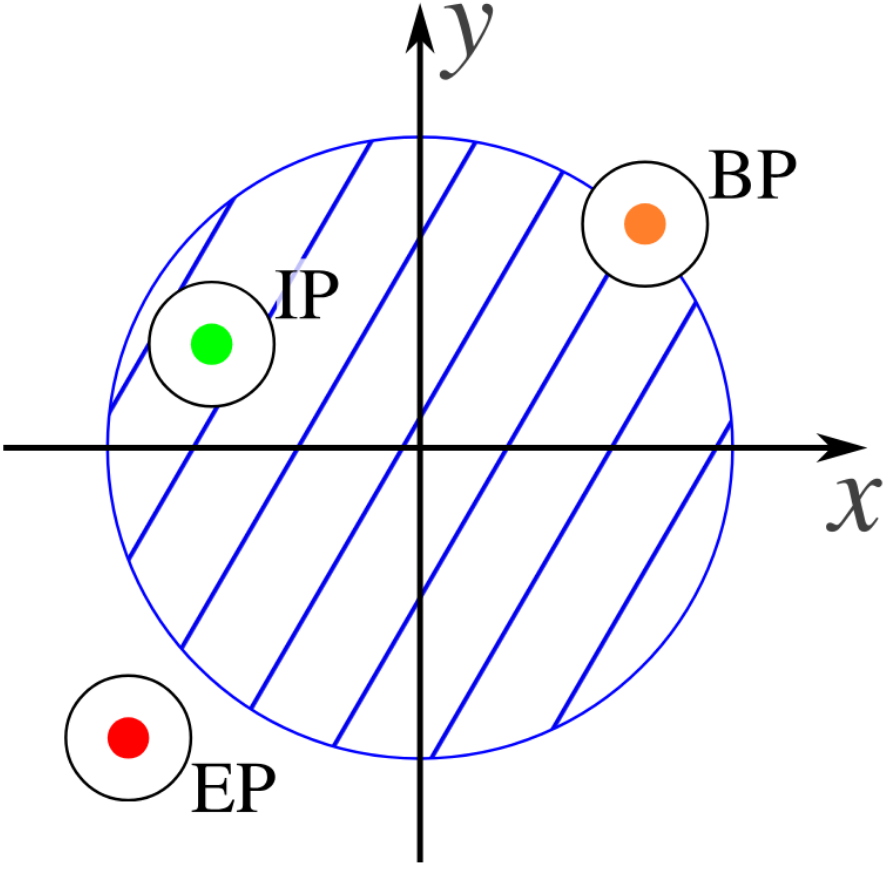
\includegraphics[width=0.5\textwidth]{ball.png}
	\caption{Interior point (IP), exterior point (EP), and boundary point (BP).}
	\label{fig:ball}
\end{figure}
Now that we have defined completeness, let us look at the difference between open and closed sets, particularly on the 2D plane. We will be considering a ball in the 2D plane,
defined,
\begin{Definitions}{Ball}{}
	A ball of radius $\epsilon$ around a point $\vb{r}_0$ is the set of all points $\vb{r}$ such that $\norm{\vb{r} - \vb{r}_0}$.
\end{Definitions} 
A sphere is the points where $\norm{\vb{r} - \vb{r}_0} = \epsilon$. Let us denote the set of the sphere $S$. We will consider three types of points, visualised in figure \ref{fig:ball},
\begin{itemize}
	\item \textbf{Exterior point}, for some $\epsilon$, all  $\vb{r} \notin S$.
	\item \textbf{Interior point}, for some $\epsilon$, all $\vb{r} \in S$.
	\item \textbf{Boundary point}, for some $\epsilon$, some of the neighbourhood of $\vb{r} \in S$ and some $\vb{r} \notin S$.
\end{itemize}
We can then define closed and open sets.
\begin{Definitions}{Closed Set}{}
	A set that contains all its boundary points is closed.
\end{Definitions}
An example of this is a set of points $\abs{r} \leq 1$, as $|r| = 1$ is a boundary point, and also belongs to the set. 
\begin{Definitions}{Open Set}{}
	A set that only includes interior points is open.
\end{Definitions}
We must furthmore define,
\begin{Definitions}{Connected Set}{}
	Sets for which any two points can be joined by a continuous path. 
\end{Definitions}
If a set is connected and open, we call it a \textit{region}.
\begin{Examples}{}{}
	The function $f(z) = \frac{1}{(1-z)}$ has a defined Taylor series for $z \neq 1$,
	\begin{equation}
		f(z) = \sum_{i=0}^{\infty}z^i.
	\end{equation}
	For what complex numbers is this series Cauchy? Is this an open or closed set?
\end{Examples}
We will consider the cases $|z| < 1$ and $|z| > 1$ separately, with $|z| =1$ as a boundary case. Let us define,
\begin{equation}
	a_n = \sum_{i=0}^n z^i.
\end{equation}
For any $z \neq 1$, assuming $n > m$,
\begin{equation}
	\abs{a_n - a_m} = \abs{\sum_{i = m+1}^n z_i } = \abs{\frac{z^{m+1}-z^{n+1}}{1-z}}.
\end{equation}
For $|z| < 1$,
\begin{equation}
	|a_n - a_m| = \frac{|z|^m}{|1-z|}\abs{1 - z^{n-m+1}}\leq \frac{2}{|1-z|}|z|^m
\end{equation}
and since $|z|^m$ is decreasing as a function of $m$, the series is Cauchy. For $|z|>1$,
\begin{equation}
	|a_n - a_m| = \frac{|z|^n}{|1-z|}\abs{1 - z^{-n+m+1}}\geq \frac{2}{|1-\frac{1}{z}|}|z|^n = z^{n+1}
\end{equation}
and since $|z|^{n}$ is an increasing function of $n$, the series is not Cauchy. Thus the series is Cauchy in the open set $|z| < 1$.
\section{Inner Product Space}
An inner product space is a vector space with an inner product, which is a generalisation of the scalar product.
\begin{Definitions}{Inner product, $\innerproduct{\vb{a}}{\vb{b}}$}{}
	Given a vector space $V_N$ over $\mathbb{F}$, the inner product between two vectors $\vb{a},\vb{b} \in V_N$ is a function such that $V \times V \to \mathbb{F}$. If $\mathbb{F} \subset \mathbb{C}$, the following properties hold,
	\begin{enumerate}
		\item \textbf{Linearity}. If $\vb{w} = \lambda\vb{u} + \mu\vb{v}$ then $\innerproduct{\vb{a}}{\vb{w}} = \lambda\innerproduct{\vb{a}}{\vb{u}} + \mu \innerproduct{\vb{a}}{\vb{u}}$.
		\item \textbf{Conjugation Symmetry.} $\overline{\innerproduct{\vb{w}}{\vb{a}}} = \innerproduct{\vb{a}}{\vb{w}}$
		\item \textbf{Positive Definiteness.} $\forall \vb{x}\neq0, \innerproduct{\vb{x}}{\vb{x}} > 0$.
	\end{enumerate}
\end{Definitions}
From our definition of the inner product, we can define the 2-norm,
\begin{equation}
	\norm{\vb{a}}^2 = \innerproduct{\vb{a}}{\vb{a}} \geq 0.
\end{equation}
\subsection{Orthogonality}
\begin{Definitions}{Orthogonality}{}
	$\forall \vb{a},\vb{b} \neq 0 \in V_N$ if $\innerproduct{\vb{a}}{\vb{b}} = 0$ then $\vb{a}$ and $\vb{b}$ are orthogonal.
\end{Definitions}
This allows us to then define an orthonormal basis.
\begin{Definitions}{Orthonormal basis}{}
	The set basis vectors $\left\{\vb{e}_i\right\}_{i=1}^N \in V_N$ is orthogonal if,
	\begin{equation}
		\innerproduct{\vb{e}_i}{\vb{e}_j} = A_i\delta_{ij}.
	\end{equation}
	and $A_i \neq 0$. The set of basis vectors is orthonormal for $A_i = 1, \forall i \in \left[1,N\right]$.
\end{Definitions}
Given we can decompose any vector $\vb{a} \in V_N$ if given a complete set of basis vectors, we can define a general inner product for $V_N$ over $\mathbb{F} \subset \mathbb{C}$. Let us begin by writing the decomposition of two vectors $\vb{a},\vb{b}\in V_N$ into a set of basis vectors $\left\{\vb{e}_j\right\}_{j=1}^N$,
\begin{align}
	\vb{a} = \sum_{j=1}^Na_j\vb{e}_j && \vb{b} = \sum_{j=1}^Nb_j\vb{e}_j.
\end{align}
Then, using linearity,
\begin{equation}
	\begin{split}
		\innerproduct{\vb{a}}{\vb{b}} & = \sum_{j,k=1}^N\overline{a}_j \innerproduct{\vb{e}_j}{\vb{e}_k}b_k \\
		& = \sum_{i,j=1}^N\overline{a}_j\delta_{jk}b_k \\
		& = \sum_{j=1}^N\overline{a}_jb_j.
	\end{split}
\end{equation}
NOTE: This only holds when using an orthonormal basis.
\\\\
We can obtain further insight into the decomposition of a vector by considering the inner product,
\begin{equation}
	\begin{split}
		\vb{a} = \sum_{j=1}^Na_j\vb{e}_j \implies \innerproduct{\vb{e}_k}{\vb{a}} & = \sum_{j=1}^Na_j\underbrace{\innerproduct{\vb{e}_j}{\vb{e}_k}}_{\delta_{jk}} = a_k.
	\end{split}
\end{equation}
We often refer to $a_k = \innerproduct{\vb{e}_k}{\vb{a}}$ as the \textit{projection} of $\vb{a}$ onto $\vb{e}_k$ as it gives the component of $\vb{a}$ in the $\vb{e}_k$ direction.
\subsection{Gram-Schmidt Orthonormalisation}
\begin{Definitions}{Gram-Schmidt Algorithm}{}
	Given a basis $\left\{\vb{v}_j\right\}_{j=1}^N \in V_N$,
	\begin{itemize}
		\item[1.] Define
		\begin{equation}
			\vb{e}_1 = \frac{\vb{v}_1}{\norm{\vb{v}_1}}
		\end{equation}
		\item[2.] Define 
		\begin{align}
			\vb{u}_2 = \vb{v}_2 - \innerproduct{\vb{e}_1}{\vb{e}_2}\vb{e_1}
	&&
			\vb{e}_2 = \frac{\vb{u}_2}{\norm{\vb{u}_2}}
		\end{align}
		\item[\vdots]
		\item[m.] Define,
		\begin{equation}
			\vb{u}_m = \vb{v}_m - \sum_{j=1}^{m-1}\innerproduct{\vb{e}_j}{\vb{v}_m}\vb{e}_j
		\end{equation}
		thus,
		\begin{equation}
			\vb{e}_m = \frac{\vb{u}_m}{\norm{\vb{u}_m}}
		\end{equation}
	\end{itemize}
	up to $N$.
\end{Definitions}
The Gram-Schmidt process is able to take any set of basis vectors and turn it into a set of orthonormal basis vectors. The idea behind it is that given 2 vectors $\vb{v},\vb{u}$ such that $\norm{\vb{u}} = 1$, then we wish to define a vector $\vb{v}' = \vb{v} - \innerproduct{\vb{u}}{\vb{v}}\vb{u}$. The inner product with $\vb{u}$ and this new vector is then,
\begin{equation}
	\innerproduct{\vb{u}}{\vb{v}'} = \innerproduct{\vb{u}}{\vb{v}} - \innerproduct{\vb{u}}{\vb{v}}\cancelto{1}{\innerproduct{\vb{u}}{\vb{u}}} = 0.
\end{equation}
So, we essentially are removing the non-orthonormal components from each subsequent basis vector, based on the first basis vector in the set.
\subsection{Inequalities of Inner Product Space}
\begin{Theorems}{Cauchy-Schwartz Inequality}{}
	$\forall \vb{a},\vb{b} \in V_N, \abs{\innerproduct{\vb{a}}{\vb{b}}} \leq \norm{\vb{a}}\norm{\vb{b}}$.
\end{Theorems}
\begin{proof}
	Consider $\vb{u} = \vb{a} - \lambda\vb{b}$,
	\begin{equation}
		\norm{\vb{a}}^2 = \norm{\vb{a}}^2 + |\lambda|^2\norm{\vb{b}}^2 - \overline{\lambda}\innerproduct{\vb{b}}{\vb{a}} - \lambda\innerproduct{\vb{a}}{\vb{b}} \geq 0.
	\end{equation}
Choose, 
\begin{equation}
	\lambda = \frac{\innerproduct{\vb{b}}{\vb{a}}}{\norm{\vb{b}}^2}.
\end{equation}
Thus,
\begin{equation}
	\begin{split}
		\norm{\vb{u}}^2 = \norm{\vb{a}}^2 \norm{\vb{b}}^2 - \frac{\abs{\innerproduct{\vb{a}}{\vb{b}}}}{\norm{\vb{b}}^2} \geq 0
	\end{split}
\end{equation}
$\implies \abs{\innerproduct{\vb{a}}{\vb{b}}} \leq \norm{\vb{a}}\norm{\vb{b}}$.
\end{proof}
\begin{Theorems}{Triangle Inequality}{}
	$\forall \vb{a},\vb{b} \in V_N, \norm{\vb{a} + \vb{b}}  \leq \norm{\vb{a}} + \norm{\vb{b}}$
\end{Theorems}
\begin{proof}
	\begin{equation}
		\begin{split}
		\norm{\vb{a} + \vb{b}}^2 & = \innerproduct{\vb{a} + \vb{b}}{\vb{a} + \vb{b}} \\
		& \leq \norm{\vb{a}}^2 + \norm{\vb{b}}^2 + 2\abs{\innerproduct{\vb{a}}{\vb{b}}} \\
		& \leq \norm{\vb{a}}^2 + \norm{\vb{b}}^2 + 2\norm{\vb{a}}\norm{\vb{b}} = (\norm{\vb{a}} + \norm{\vb{b}})^2
		\end{split}
	\end{equation}
	$\implies \norm{\vb{a} + \vb{b}} \leq \norm{\vb{a}} + \norm{\vb{b}}$
\end{proof}
\section{Function Space}
We denote function spaces by $\mathcal{F}$. Let us define the function space inner product.
\begin{Definitions}{Function Space Inner Product}{}
	For $x \in \left[a,b\right]$, and functions $f,g : \left[a,b\right] \to \mathbb{C}$, the inner product is given by
	\begin{equation}
		\braket{f}{g} = \int_a^b\overline{f(x)}g(x)\dd\mu(x)
	\end{equation}
	where $\dd\mu(x)$ is the integration measure of a function space.
\end{Definitions}
The inner product must satisfy,
\begin{equation}
	\norm{f}^2 = \braket{f}{f} = \int_a^b |f(x)|^2\dd\mu(x) \geq 0
\end{equation}
which is only 0 if $f(x) = 0 \forall x$. If $\norm{f}^2$ is finite, then $f$ is square-integrable and can be normalised. Function spaces where all functions are square-integrable are known as Hilbert spaces.
\begin{Definitions}{L2 Functions}{}
	A function $f$ is said to be in the space $L^2(\left[a,b\right])$ if $\norm{f}^2 = \int_a^b|f(x)|^2\dd\mu(x) < \infty$.
\end{Definitions}
Let us note that we will use $\dd\mu(x) = \dd{x}$ throughout the course, however most concepts can be generalised to an arbitrary measure.
\subsection{Basis functions and completeness}
A function $f \in \mathcal{F}$ over the domain $x \in \left[a,b\right]$ can be represented by a set of basis vectors $\left\{u_n\right\}_{n=1}^{\infty} \in \mathcal{F}$ as,
\begin{equation}
	f(x) = \sum_{n=1}^{\infty}f_nu_n(x)
\end{equation}
where the coefficients $f_n$ are defined,
\begin{equation}
	f_n = \braket{u_n}{f} = \int_a^b\overline{u_n(x)}f(x)\dd{x}.
\end{equation}
We can define the completeness relation for an infinite function space by,
\begin{equation}
	\sum_{n=1}^{\infty}u_n(x) \overline{u_n(y)} = \delta(x-y).
\end{equation}
\subsection{Coordinate Representation}
When we write $f(x)$, we are referring to a function $f \in \mathcal{F}$ in a basis defined by the coordinate $x$. Let us write this more explicitly, calling $\ket{x}$ the \textit{position vector}, and writing $f \in \mathcal{F}$,
\begin{equation}
	\ket{f} = \int_a^b\dd{x}f(x)\ket{x}
\end{equation}
where we integrate rather than sum since position is continuous. We can then clearly see,
\begin{equation}
	f(x) = \braket{x}{f} = \int_a^b\delta(y-x)f(y)\dd{y}
\end{equation}
from which we find that the Dirac-delta acts as a basis vector for position vectors. We define the overlap of two position vectors,
\begin{equation}
	\braket{x}{x'} = \int_a^b\delta(y-x)\delta(y-x')\dd{y} = \delta(x-x') \iff x,x'\in\left[a,b\right].
\end{equation}
The completeness relation is then,
\begin{equation}
	\int_a^b\ket{x}\bra{x}\dd{x} = \hat{\mathbb{1}}.
\end{equation}
\chapter{Linear Operators}
\begin{Definitions}{Map}{}
	A map $M$ is a function which takes $V \to W$ where $V,W$ are vector spaces. This is such that $M$ acting on $\vb{c} \in V$ produces a different vector $\vb{c}' \in W$.
\end{Definitions}
We are often interested in linear maps, or linear operators as they are often called in physics.
\begin{Definitions}{Linear Operator}{}
	An operator $\hat{A}$ is linear if, for a vector $\vb{c} = \lambda \vb{a} + \mu\vb{b}$ where $\forall \lambda, \mu \in \mathbb{F}$ and $\forall \vb{a},\vb{b} \in V$ over $\mathbb{F}$, 
	\begin{equation}
		\vb{c}' = \hat{A}\vb{c} = \mu(\hat{A}\vb{a})+ \lambda (\hat{A}\vb{b})
	\end{equation}
\end{Definitions}
In physics, but not generally, linear operators always map $V \to V$.
\section{Algebra of operators}
We can define the following properties of linear operators,
\begin{enumerate}
	\item $(\hat{A} + \hat{B}) \equiv \hat{A}\vb{v} + \hat{B} \vb{v}$.
	\item $(\lambda\hat{A})\vb{v} = \lambda(\hat{A}\vb{v})$.
	\item $\exists\hat{\mathbb{1}} : \hat{\mathbb{1}}\vb{v} = \vb{v}, \forall \vb{v} \in V$.
	\item $\exists \hat{0} : \hat{0}\vb{v} = \vb{0}, \forall \vb{v} \in V$.
	\item $\forall \vb{v} \in V, (\hat{B}\hat{A})\vb{v} = \hat{B}(\hat{A}\vb{v})$, generally $\hat{A} \hat{B} \neq \hat{B}\hat{A}$
\end{enumerate}
\section{Matrix Representation of Linear Operators}
Consider $V_N$ over $\mathbb{F}$. Assume $\left\{\vb{e}_j\right\}_{j=1}^N$ is an orthonormal basis. $\forall \vb{v} \in V_N$,
\begin{equation}
	\vb{v} = \sum_{j=1}^Nv_j \vb{e}_j
\end{equation}
where $\innerproduct{\vb{e}_k}{\vb{v}} = v_k$. Given a linear operator $\hat{A}$,
\begin{equation}
	\hat{A} \vb{v} = \hat{A} \left(\sum_{j=1}^N v_j\vb{e}_j\right) = \sum_{j=1}^Nv_j\hat{A}\vb{e}_j
\end{equation}
by linearity. We have $\hat{A}\vb{e}_j \in V_N$, thus,
\begin{equation}
	\hat{A} \vb{e}_j = \sum_{i=1}^N\vb{e}_i\underbrace{(\hat{A}\vb{e}_j)}_{A_{ij}}
\end{equation}
so,
\begin{equation}
	\begin{split}
		& \hat{A}\vb{e}_j = \sum_{i=1}^N\vb{e}A_{ij} \\
		\implies & A_{ij} = \innerproduct{\vb{e}_i}{\hat{A}\vb{e}_j}.
	\end{split}
\end{equation}
So,
\begin{equation}
	\begin{split}
		\hat{A}\vb{v} & = \sum_{j=1}^Nv_j\sum_{i=1}^N(A_ij\vb{e}_i) \\
		& =\sum_{i=1}^{N}\left(\sum_{j=1}^NA_{ij}v_j\right)\vb{e}_i
	\end{split}
\end{equation}
thus,
\begin{equation}
	(\hat{A}\vb{v})_i = \sum_{j=1}^N A_{ij}v_j.
\end{equation}
Interestingly, we have obtained matrix multiplication from linearity and orthonormality, rather than having to define it.
\section{Inverse Operator}
\begin{Definitions}{Inverse operator}{}
	Given an operator $\hat{A}$ from $V \to V$, $\forall \vb{v} \in V$, $\exists \hat{B}$ such that, $\hat{B}(\hat{A}\vb{v}) = \vb{v}$, $(\hat{B}\hat{A})\vb{v} = \vb{v} \implies \hat{B}\hat{A} = \hat{\mathbb{1}}$. We call $\hat{B} = \hat{A}^{-1}$.
\end{Definitions}
NOTE: Not all operators have an inverse.
\section{Dyadic (Outer) Product}
Recall $\bra{u}\hat{A}\ket{v} \to$ $\vb{u}^{\dag}\hat{A}\vb{v}$, or $\innerproduct{\vb{u}}{\hat{A}\vb{v}}$. We can clearly see that $\vb{c}\innerproduct{\vb{a}}{\vb{b}}$ is a vector. Let us define,
\begin{equation}
	\vb{c}' = \vb{c}(\vb{a}^{\dag}\vb{b}) = \underbrace{(\vb{c}\vb{a}^{\dag})}_{\substack{\text{Linear}\\\text{Operator}}}\vb{b}
\end{equation}
this linear operator is known as a \textit{dyad} or the \textit{outer product} of $\vb{a}$ and $\vb{c}$. Let us define it more formall,y

\begin{Definitions}{Dyad/Outer product}{}
	For $V_N \subset \mathbb{C}^N$, and vectors $\vb{a},\vb{b} \in V_N$, their outer product is defined $\vb{a}\vb{b}^{\dag}$. It has the following properties,
	\begin{enumerate}
		\item \textbf{Linearity in the first argument}. If $\vb{c} = \lambda \vb{a} + \mu \vb{b}$, then $\vb{c}\vb{d}^{\dag} = \lambda\vb{a}\vb{d}^{\dag} + \mu\vb{b}\vb{d}^{\dag}$.
		\item \textbf{Antilinearity in the second argument}. If $\vb{d} = \lambda \vb{a} + \mu \vb{b}$, then $\vb{c}\vb{d}^{\dag} = \bar{\lambda}\vb{c}\vb{a}^{\dag} + \bar{\mu}\vb{c}\vb{b}^{\dag}$.
	\end{enumerate}
\end{Definitions}
\section{Projection Operator and the Completeness Relation}
If $\hat{P}^2\vb{v} = \hat{P}\vb{v}$, $\forall \vb{v} \in V_N$, then $\hat{P}$ is a projection operator. For a given orthonormal basis $\left\{\vb{e}_j\right\}_{j=1}^N \in V_N$, $\hat{P}_j = \vb{e}_j\vb{e}_j^{\dag}$. A consequence of this is the completeness relation, 
\begin{equation}
	\sum_{j=1}^N\hat{P}_j = \sum_{j=1}^N \vb{e}_j\vb{e}_j^{\dag} = \hat{\mathbb{1}}.
\end{equation}
\section{The Adjoint or Hermitian Conjugate}
\begin{Definitions}{Adjoint}{}
	\begin{equation}
	\forall \hat{A}, \forall \vb{u},\vb{v} \in V_N : \innerproduct{\vb{u}}{\hat{A}^{\dag}\vb{v}} = \overline{\innerproduct{\vb{v}}{\hat{A}\vb{u}}}
\end{equation}
In matrix notation,
\begin{equation}
	(\hat{A}^{\dag})_{ij} = \overline{A_{ji}}.
\end{equation}
An operator is self adjoint if $\hat{A} = \hat{A}^{\dag}$.
\end{Definitions}
\begin{Definitions}{Unitary Operator}{}
	\begin{equation}
		\exists \hat{U} : \hat{U}^{\dag}\hat{U} = \hat{U}\hat{U}^{\dag} = \hat{\mathbb{1}}
	\end{equation}
	i.e.,
	\begin{equation}
		\hat{U}^{-1} = \hat{U}^{\dag}.
	\end{equation}
\end{Definitions}

\section{Representations}
\subsection{Representation of a Vector}
We know that a vector can be decomposed into orthonormal basis vectors. A vector space can have more than one set of orthonormal basis vectors which can represent a given vector. From the completeness relation, we find,
\begin{equation}
	\begin{split}
		\vb{v} = \hat{\mathbb{1}}\vb{v} &= \sum_{j=1}^N \innerproduct{\vb{e}_j}{\vb{v}}\vb{e}_j \\ 
		& = \sum_{j=1}^N\innerproduct{\vb{f}_j}{\vb{v}}\vb{f}_j
	\end{split}
\end{equation}
i.e., changing basis does not change the abstract concept of a vector.
\subsubsection{Invariance of the Inner Product}
We can emphasise the idea above by considering the inner product of a vector. We can write some vector $\vb{v}\in V_N$ as,
\begin{equation}
	\vb{v} = \sum_{j=1}^Na_i\vb{e}_i = \sum_{j=1}^N b_i\vb{f}_i.
\end{equation}
Computing the inner product,
\begin{equation}
	\begin{split}
	\innerproduct{\vb{v}}{\vb{v}} & = \sum_{j=1}^N\left(a_j\vb{e}_j\right)^{\dag}\sum_{k=1}^Na_k\vb{e}_k \\
	& = \sum_{j=1}^N\sum_{k=1}^N\overline{a_j}a_k\underbrace{\vb{e}_j^{\dag}\vb{e}_k}_{\delta_{jk}} \\
	& = \sum_{j=1}^N\abs{a_j}^2
	\end{split}
\end{equation}
and repeating this using the $\left\{\vb{f}_j\right\}_{j=1}^N$ representation,
\begin{equation}
	\begin{split}
		\innerproduct{\vb{v}}{\vb{v}} & = \sum_{j=1}^N\left(b_j\vb{f}_j\right)^{\dag}\sum_{k=1}^Nb_k\vb{f}_k \\
		& = \sum_{j=1}^N\abs{b_j}^2
	\end{split}
\end{equation}
and we find $\sum_{j=1}^N\abs{a_j}^2 = \sum_{j=1}^N\abs{b_j}^2$, so the inner product is invariant under a basis change.
\subsection{Representation of Linear Operators}
Consider a vector space $V_N$ with basis $\left\{\vb{e}_j\right\}_{j=1}^N$. Consider $\vb{b},\vb{c} \in V_N$ and an operator $\hat{A}$, such that $\vb{c} = \hat{A}\vb{b}$. We can find its representation by considering,
\begin{equation}
	\begin{split}
		\mathbb{1} \vb{c} = \mathbb{1} \hat{A}\mathbb{1}\vb{b} & \\
		\sum{j=1}^N \innerproduct{\vb{e}_j}{\vb{c}} \vb{e}_j & = \sum_{j,k=1}^N\left(\vb{e}_j\vb{e}_j^{\dag}\right)\hat{A}\left(\vb{e}_k\vb{e}_k^{\dag}\right)\vb{b} \\
		& = \sum_{j,k=1}^N \vb{e}_j\underbrace{\left(\vb{e}_j^{\dag}\hat{A}\vb{e}_k\right)}_{A_{ij}}\underbrace{\left(\vb{e}_k^{\dag}\vb{b}\right)}_{b_k}
	\end{split}
\end{equation}
Thus, we find that we can denote the entries of a matrix $\doubleunderline{A}$ representing a linear operator $\hat{A}$ are $\left(\doubleunderline{A}\right)_{ij}$. We can denote this representation by,
\begin{align}
	\hat{A} \xrightarrow{\left\{\vb{e}\right\}_{j=1}^N} \doubleunderline{A}.
\end{align}
\subsection{Changing Representation of a Vector}
Consider a vector $\vb{v} \in V_N$, and orthonormal bases $\left\{\vb{e}_j\right\}_{j=1}^N$ and $\left\{\vb{f}_j\right\}_{j=1}^N$. $\vb{v}$ can be decomposed as,
\begin{equation}
		\vb{v} = \sum_{j=1}^Na_i\vb{e}_i = \sum_{j=1}^N b_i\vb{f}_i.
\end{equation}
The $l^{\text{th}}$ element of the vector is given by,
\begin{equation}
	a_l = \innerproduct{\vb{e}_l}{\vb{v}} = \sum_{k=1}^Nb_k\innerproduct{\vb{e}_l}{\vb{f}_k} = \sum_{k=1}^N\left(\doubleunderline{U}_{lk}\right)b_k
\end{equation}
where we have found the matrix $(\doubleunderline{U})_{lk}$ which represents a unitary operator that takes a vector representation from one basis and transforms it into another. We can denote this,
\begin{equation}
	\begin{pmatrix}
		a_1 \\ a_2 \\ \vdots \\ a_N
	\end{pmatrix} = \begin{pmatrix}
	\innerproduct{\vb{e}_1}{\vb{f}_1} & \cdots & \innerproduct{\vb{e}_1}{\vb{f}_N} \\
	\innerproduct{\vb{e}_2}{\vb{f}_1} & \cdots & \innerproduct{\vb{e}_2}{\vb{f}_N} \\
	\vdots & \ddots & \vdots \\
	\innerproduct{\vb{e}_N}{\vb{f}_1} & \cdots & \innerproduct{\vb{e}_N}{\vb{f}_N}
	\end{pmatrix}\begin{pmatrix}
	b_1 \\ b_2 \\ \vdots \\ b_N
	\end{pmatrix}
\end{equation} 
\subsection{Changing Representation of a Matrix}
We can write a linear operator as,
\begin{equation}
	\hat{A} = \mathbb{1}\hat{A} \mathbb{1} = \sum_{j,k=1}^NA_{jk}\vb{e}_j\vb{e}_k^{\dag} = \sum_{l,m=1} \tilde{A}_{lm}\vb{f}_l\vb{f}_m^{\dag}
\end{equation}
we then find that,
\begin{equation}
	A_{jk} = \sum_{l,m=1}^N \innerproduct{\vb{e}_j}{\vb{f}_l}\tilde{A}_{lm}\innerproduct{\vb{f}_m}{\vb{e}_k}.
\end{equation}
Thus, we find that we can change the matrix representation of a linear operator by,
\begin{equation}
	\doubleunderline{A} = \doubleunderline{U}\doubleunderline{\tilde{A}}\doubleunderline{U}^{\dag}.
\end{equation}
\section{Eigenvalue Problems}
\begin{Definitions}{Eigen Equation}{}
	For a linear operator $\hat{A}$, the eigenequation is,
	\begin{equation}
		\hat{A}\vb{u}= \lambda \vb{u}
	\end{equation}
	where $\lambda$ and $\vb{u}$ are the eigenvalue and right eigenvector of $\hat{A}$ respectively, such that $\vb{u} \neq \vb{0}$.
\end{Definitions}
A left eigenvector will satisfy,
\begin{equation}
	\vb{v}^{\dag}\hat{A} = \lambda\vb{v}^{\dag}.
\end{equation}
In order to obtain the eigenvalues, we rearrange to get,
\begin{equation}
	\left(\hat{A} - \lambda \hat{\mathbb{1}}\right)\vb{u} = 0
\end{equation}
and solve,
\begin{equation}
	\det\left(\hat{A} - \lambda \hat{\mathbb{1}}\right)
\end{equation}
which generates a polynomial of degree $N$, with $N$ solutions for $\lambda in \mathbb{C}$. Each distinct eigenvalue will correspond to a distinct eigenvector. However, if we have a repeated root, we get repeated eigenvectors. For $m > 1$ repeated eigenvectors, there may be up to, but at least 1, $m$ linearly independent eigenvectors corresponding to the degenerate eigenvalue. 
\subsection{Eigenvalues and eigenvectors of Hermitian operators}
\begin{Theorems}{Eigenvalues of Hermitian Operators}{}
	Consider the eigenvalues $\left\{\lambda_i\right\}_{i=1}^N$ and eigenvectors $\left\{\vb{u}\right\}_{i=1}^N$ of $\hat{A}$. $\forall \hat{A} : \hat{A}^{\dag} = \hat{A} \implies \forall i: \lambda_i \in \mathbb{R}$, $\forall i\neq j: \vb{u}_i^{\dag}\vb{u}_j = 0$.
\end{Theorems}
\begin{proof}
	The eigenvalue equation is given by,
	\begin{equation}
		\hat{A}\vb{u}_i = \lambda_i \vb{u}_i.
	\end{equation}
	Without loss of generality, consider the matrix elements of $\hat{A}$ with respect to two eigenvectors,
	\begin{equation}
		\vb{u}_j^{\dag}\hat{A}\vb{u}_k = \lambda_k\innerproduct{\vb{u}_j}{\vb{u}_k}. \label{eq:1}
	\end{equation}
	Using the Hermitian property,
	\begin{equation}
		\vb{u}_j^{\dag}\hat{A}\vb{u}_k = \vb{u}_j^{\dag}\hat{A}^{\dag}\vb{u}_k = \overline{\vb{u}_k^{\dag}\hat{A}\vb{u}_j} = \overline{\lambda_j}\left<\vb{u}_j, \vb{u}_k\right>. \label{eq:2}
	\end{equation}
	Equating equations \eqref{eq:1} and \eqref{eq:2},
	\begin{equation}
		(\lambda_k - \overline{\lambda}_k)\innerproduct{\vb{u}_j}{\vb{u}_k} = 0.
	\end{equation}
	Let us consider two cases,
	\begin{enumerate}
		\item $k = j$, since $\innerproduct{\vb{u}_j}{\vb{u}_j} > 0$, we require $\lambda_j = \overline{\lambda}_j$. 
		\item $k\neq j$, since $\lambda_j, \lambda_k$ are distinct, we require $\innerproduct{\vb{u}_j}{\vb{u}_k} = 0$. 
	\end{enumerate}
\end{proof}
\subsection{Diagonalisation}
Let $\doubleunderline{U}$ be the matrix with orthonormal eigenvectors $\vb{u}_j$ as columns, such that $U_{ij} = (u_j)_i$, and $\hat{U}$ be the corresponding linear operator. By orthogonality, $\hat{U}$ is unitary. For a linear operator $\hat{A}$, we can diagonalise it (construct a matrix with $\hat{A}$'s eigenvalues on the diagonal) by,
\begin{equation}
	\left[\hat{U}^{\dag}\hat{A}\hat{U}\right]_{ij} = \lambda_i\delta_{ij}.
\end{equation}
To obtain the original operator form its diagonalised form $\Lambda_{ij}$, we perform,
\begin{equation}
	A_{ij} = U_{ik}\Lambda_{kl}\overline{U}_{jl}.
\end{equation}
\subsubsection{Eigenvalues and eigenvectors of unitary operators}
We use unitary operators in physics to describe time evolution in quantum mechanics. We can do this because they preserve the norm, and thus the inner product, of a vector. i.e., $\innerproduct{\hat{U}\vb{u}}{\hat{U}\vb{v}} = \innerproduct{\vb{u}}{\vb{v}}$.
\begin{Theorems}{Eigenvalues of unitary operators}{}
	Consider a unitary operator $\hat{U} : V \to V$ with eigenvalue equation,
	\begin{equation}
		\hat{U}\vb{u}_j = \lambda_j\vb{u}_j.
	\end{equation}
	The eigenvalues satisfy the following condition:
	\begin{enumerate}
		\item $\abs{\lambda_j} = 1 \implies \lambda_j = e^{i\theta_j}, \theta \in \mathbb{R}$.
		\item $\lambda_j \neq \lambda_k \implies \innerproduct{\vb{u}_j}{\vb{u}_k} = 0$.
		\item The eigenvectors of $\hat{U}$ form an orthonormal basis for $V$.
	\end{enumerate}
\end{Theorems}
\begin{proof}
	\begin{enumerate}
		\item We need to prove that $\abs{\lambda_j}^2 = 1$. Consider the left anr right eigenequations of $\hat{U}$,
		\begin{align}
			\hat{U}\vb{u}_j &= \lambda\vb{u}_j\\
			\vb{u}_j^{\dag}\hat{U}^{\dag} & = \overline{\lambda_j} \vb{u}_j^{\dag}
		\end{align}
		from which we find,
		\begin{equation}
			\begin{split}
			\vb{u}_j^{\dag}\hat{U}^{\dag}\hat{U}\vb{u}_j & = \vb{u}^{\dag}\hat{\mathbb{1}}\vb{u} = \overline{\lambda}\lambda\vb{u}^{\dag}_j\vb{u}_j \\
			& = \vb{u}^{\dag}\vb{u} = |\lambda|^2\vb{u}_j^{\dag}\vb{u} \\
			& \implies \left(1 - |\lambda|^2\right)\vb{u}^{\dag}_j\vb{u}_j
			\end{split}
		\end{equation}
		we have $\vb{u} \neq \vb{0}$, so we require $|\lambda|^2 = 1$, and thus $\lambda = e^{i\theta}, \theta \in \mathbb{R}$.
		\item Let us consider the left and right eigenequations again. We have,
		\begin{equation}
			\begin{split}
				\vb{u}_j^{\dag}\vb{u}_k & = \overline{\lambda_j}\lambda_k\vb{u}_j^{\dag}\vb{u}_k \\
				\implies \innerproduct{\vb{u}_j}{\vb{u}_k}(1 - \overline{\lambda_j}\lambda_k) & = 0
			\end{split}
		\end{equation}
		we require $\overline{\lambda_j}\lambda_k \neq 1, \forall j \neq k, \therefore \innerproduct{\vb{u}_j}{\vb{u}_k}$.
		\item For completeness, we must write $\vb{v} = \sum_{j=1}^Nc_j\vb{u}_j$. We have shown $\left\{\vb{u}_j\right\}_{i=1}^N$ to be orthonormal, so we can write,
		%\begin{equation}
			$c_j = \innerproduct{\vb{u}_j}{\vb{v}}$.
		%\end{equation}
	\end{enumerate}
\end{proof}
\subsubsection{Spectral Representation}
We can diagonalise a general operator $\hat{A}$ which is not necessarily Hermitian, under the assumption that it has a complete set of eigenvectors. The left and right eigenvector equations are,
\begin{align}
	\vb{v}_j^{\dag}\hat{A} = \lambda_j\vb{v}_j^{\dag} && \hat{A}\vb{u}_j = \lambda_j\vb{u}_j.
\end{align}
We then have,
\begin{equation}
	\vb{v}_j^{\dag}\hat{A}\vb{u}_k = \lambda_k\innerproduct{\vb{v}_j}{\vb{u}_k} = \lambda_j\innerproduct{\vb{v}_j}{\vb{u}_k}
\end{equation}
thus for $\lambda_j \neq \lambda_k$, we require $\innerproduct{\vb{v}_j}{\vb{u}_k} = 0$.
\\\\
We choose a normalisation $\innerproduct{\vb{v}_j}{\vb{u}_k}$, the completeness relation is given by,
\begin{equation}
	\sum_{j=1}^N \vb{u}_j\vb{v}_j^{\dag} = \hat{\mathbb{1}}
\end{equation}
and we call $\vb{v}_j$ the dual basis to $\vb{u}_j$. We can thus write the operator $\hat{A}$,
\begin{equation}
	\boxed{\hat{A} = \hat{A}\hat{\mathbb{1}} = \sum_{j=1}^N\hat{A}\vb{u}_j\vb{v}_j^{\dag} = \sum_{j=1}^N\lambda_j\vb{u}_j\vb{v}_j^{\dag}}
\end{equation}
which is known as the \textit{spectral representation} of $\hat{A}$. Given an orthonormal basis $\left\{\vb{e}_j\right\}_{j=1}^N$ in which we can write the matrix representation of $\hat{A}$ which we denote $\doubleunderline{A}$, we can diagonalise it by applying,
\begin{equation}
	\doubleunderline{A}^{\text{diag}} = \doubleunderline{S} \doubleunderline{A} \doubleunderline{T}^{\dag}
\end{equation}
where we define,
\begin{align}
	\left(\doubleunderline{S}\right)_{jk} = \innerproduct{\vb{v}_j}{ \vb{e}_k} && \left(\doubleunderline{T}\right)_{jk} = \innerproduct{\vb{u}_j}{\vb{e}_k}
\end{align}
which are unitary only if $\hat{A}$ is Hermitian.
\subsubsection{Diagonalisation of commuting operators}
For two commuting operators $\hat{A}$ and $\hat{B}$, when,
\begin{equation}
	\hat{B} \vb{u} = \lambda \vb{u}
\end{equation}
we have,
\begin{equation}
	\begin{split}
		& \hat{A}\hat{B}\vb{u} = \lambda\hat{A}\vb{u} \\
		\implies & \hat{B}\hat{A} = \lambda \left(\hat{A}\vb{u}\right)
	\end{split}
\end{equation}
and thus $\hat{A}\vb{u}$ is also an eigenvector of $\hat{B}$ with eigenvalue $\lambda$. Below the implications of this statement are stated,
\begin{itemize}
	\item \textbf{Non-degenerate:} If $\lambda$ is non-degenerate, $\forall\lambda, \exists\vb{u} : \hat{A}\vb{u} = \mu\vb{u} \implies$ $\vb{u}$ is a simultaneous eigenvector of $\hat{B}$ and $\hat{A}$.
	\item \textbf{Degenerate:} If $\lambda$ has degeneracy $m > 1$, with eigenvectors $\left\{\vb{u}_j\right\}_{j=1}^m$, then a linear combination of these eigenvectors is an eigenvector of $\hat{A}$. $\hat{B}$ will act in this subspace, and it is possible to find a basis which simultaneously diagonalises $\hat{A}$ and $\hat{B}$.
\end{itemize}
\section{Functions of Operators}
We wish to apply functions such as $\exp(\hat{A})$ to linear operators, and more generally functions such as $f$. 
\subsection{Taylor Expansion about 0}
We have well defined multiplication and addition on operators, so we can construct a Taylor series to define a function of an operator in most cases.
\begin{Definitions}{$f(\hat{A})$}{}
	For $f : \mathbb{C} \to \mathbb{C}$, with a Taylor series about $0$,
	\begin{equation}
		f(z) = \sum_{n=0}^{\infty}\frac{f^{(n)}(0)}{n!}z^n
	\end{equation}
	we define the composition of the function and an operator $\hat{A}$ by the same series,
	\begin{equation}
		f(\hat{A}) = \sum_{n=0}^{\infty}\frac{f^{(0)}}{n!}\hat{A}^n.
	\end{equation}
\end{Definitions}
where,
\begin{align}
	f^{(n)}(0) = \eval{\dv[n]{f(0)}{x}}_{0} && \hat{A}^n = \underbrace{\hat{A}\hat{A}\ldots\hat{A}}_{n\text{ times}}
\end{align}
\subsection{Spectral Decomposition}
Given $\hat{A}$ is diagonalisable, let us apply $f(\hat{A})$ to an eigenvector $\vb{u}$ of $\hat{A}$ with eigenvalue $\lambda$, assuming $f$ has a Taylor series,
\begin{equation}
	\begin{split}
		f(\hat{A})\vb{u} & = \sum_{n=0}^{\infty}\frac{f^{(n)}(0)}{n!}\hat{A}^n\vb{u} \\
		& = f(0) \vb{u} + \sum_{n=1}^{\infty}\frac{f^{(n)}(0)}{n!}\hat{A}^{n-1}\lambda^n\vb{u} \\
		& = \sum_{n=0}^{\infty}\frac{f^{(n)}(0)}{n!}\lambda^n\vb{u} = f(\lambda)\vb{u}.
	\end{split}
\end{equation}
If the eigenbasis of $\hat{A}$ is complete, we are able to work in it to represent $f(\hat{A})$ as,
\begin{equation}
	f(\doubleunderline{A}) = \text{diag}\left(\left\{f(\lambda_j)\right\}_{j=1}^N\right)
\end{equation}
where $\text{diag}$ is a function which constructs a matrix with the values in its arguments on the diagonal, and 0s in all other elements. We can then construct the final operator,
\begin{equation}
	f(\hat{A}) = \sum_{i=1}^Nf(\lambda_i) f(\lambda_i)\vb{u}_i\vb{v}_i^{\dag}
\end{equation}
where $\vb{v}_i^{\dag} = \vb{u}_i^{\dag}$ for a Hermitian operator.
\subsection{Time Evolution Operator}
\begin{Theorems}{Unitary operators as exponentials}{}
	For a Hermitian operator $\hat{A}$, then,
	\begin{equation}
		\hat{U}(\theta) = \exp(-i\hat{A}\theta) \label{eq:timeev}
	\end{equation}
	where $\theta \in \mathbb{R}$, is also unitary.
\end{Theorems} 
\begin{proof}
	Considering the spectral representation of $\hat{A}$, with eigenvalues $\lambda_j$ and eigenvectors $\vb{u}_j$, such that $\hat{A} = \sum_{j=1}^N\lambda_j\vb{u}_j\vb{u}_j^{\dag}$ then,
	\begin{equation}
		\hat{U}(\theta) = \sum_{j=1}^N\exp(-i\lambda_j\theta) \vb{u}_j\vb{u}_j^{\dag}.
	\end{equation}
	The adjoint $\hat{U}^\dag(\theta)$ is,
	\begin{equation}
		\hat{U}^{\dag}(\theta) = \sum_{j=1}^N\exp(i\lambda_j\theta) \vb{u}_j\vb{u}_j^{\dag}
	\end{equation}
	we then find,
	\begin{equation}
		\begin{split}
			\hat{U}^\dag(\theta)\hat{U}(\theta) & = \sum_{j,k}e^{-i(\lambda_j - \lambda_k)\theta}\vb{u}_k\vb{u}_k^{\dag}\vb{u}_j\vb{u}_j^{\dag} = \sum_{jk}e^{-i(\lambda_j - \lambda_k)\theta}\vb{u}_k^{\dag}\innerproduct{\vb{u}_k}{\vb{u}_j}\vb{u}_j \\
			& = \sum_{jk}e^{-i(\lambda_j - \lambda_k)\theta}\vb{u}_k^{\dag}\delta_{kj}\vb{u}_j = \sum_j \vb{u}_j\vb{u}_j^{\dag} = \hat{\mathbb{1}}.
		\end{split}
	\end{equation}
	thus the operator is unitary.
\end{proof}
Furthermore, the operator in equation \eqref{eq:timeev} is the time-evolution operator in quantum mechanics, where we would replace $\hat{A}$ with $\hat{H}$ and $\theta$ with $t$.
\subsection{Overlap Matrix}
We wish to develop an alternative method to the Gram-Schmidt process, and will allow us to generalise some things. Let us suppose we have a set of vectors $\left\{\vb{v}_j\right\}_{j=1}^M$ in a vector space $V_N$. We will \textbf{not} assume that $M \leq N$. The matrix overlap is given by,
\begin{equation}
	\hat{N} = \sum_{i=1}^M\vb{v}_i\vb{v}_i^{\dag}
\end{equation}
which is Hermitian, and whose matrix representation can be written,
\begin{equation}
	N_{kl} = \sum_{i=1}^Mv_{ik}\overline{v}_{il}.
\end{equation}
If we are given normalised eigenvectors $\vb{u}$ and eigenvalues of $\hat{N}$, we find,
\begin{equation}
	\vb{u}_k^{\dag}\hat{N}\vb{u}_k = \lambda_k = \sum_{i=1}^N\abs{\innerproduct{\vb{v}_i}{\vb{u}_k}}^2 \geq 0
\end{equation}
so, all of its eigenvalues must be either positive or 0. If all eigenvalues are positive, we find the inverse of the overlap matrix by writing it in the orthonormal basis $\left\{\vb{u}_j\right\}_{j=1}^M$,
\begin{equation}
	\hat{N}^{-1} = \sum_{i=1}^M\lambda_i^{-1}\vb{u}_i\vb{u}_i^{\dag}.
\end{equation}
For the case that we have a zero eigenvalue, we can define a \textit{pseudo-inverse}.
\begin{Definitions}{Pseudo-inverse}{}
	For a Hermitian operator $\hat{N}$ with a set of eigenvalues $\left\{\lambda_i\right\}_{i=1}^{M}$ and a set of normalised eigenvectors $\left\{\vb{u}\right\}_{i=1}^M$, the pseudo-inverse is defined,
	\begin{equation}
		\hat{N}_{+}^{-1} = \sum_{i=1}^{M'}\frac{1}{\lambda_{i}^+}\vb{u}_i\vb{u}_i^{\dag}
	\end{equation}
	where $\left\{\lambda_{i,+}\right\}_{i=1}^{M'} \subset \left\{\lambda_i\right\}_{i=1}^{M}$ containing only the positive eigenvalues of $\hat{N}$, with size $M' < M$.
\end{Definitions}
We can now extract an orthonormal basis from $\vb{v}$. We define the inverse square root operator of the overlap matrix as,
\begin{Definitions}{Inverse square root operator}{}
	\begin{equation}
		\hat{N}_{+}^{-1/2} = \sum_{i=1}^{M'}\frac{1}{\sqrt{\lambda^+}}\vb{u}_i\vb{u}_i^{\dag}.
	\end{equation}
\end{Definitions}
If there is a basis, we must have $N$ non-zero eigenvalues, so $M' = N$. We clearly see,
\begin{equation}
	\vb{e}_i = \hat{N}_+^{-1/2}\vb{v}_i
\end{equation}
are orthonormal vectors, and can be used as an $N$-dimensional basis. We can then find the matrix representation of any operator in this basis, where it is given in a representation $\hat{A} \xrightarrow{\left\{\vb{v}_i\right\}_{i}^M} \doubleunderline{A}$ and $\left\{\vb{v}_i\right\}_{i}^M$ is a non-basis, as,
\begin{equation}
	\tilde{\doubleunderline{A}} = \doubleunderline{N_{+}^{-1/2}}\doubleunderline{A}\doubleunderline{N_{+}^{-1/2}}
\end{equation}
\section{The Trace}
\begin{Definitions}{The Trace}{}
	Consider an operator $\hat{A}$ which acts on a vector space $V_N$. For a given orthonormal basis $\left\{\vb{e}_j\right\}_{j=1}^N$, the trace of $\hat{A}$ is the sum of its diagonal elements,
	\begin{equation}
		\Tr(\hat{A}) = \sum_{j=1}^N\vb{e}_j^{\dag}\hat{A}\vb{e}_j.
	\end{equation}
\end{Definitions}
The trace is independent of basis. We define several properties of the trace below,
\begin{enumerate}
	\item \textit{Linearity}: $\Tr(\alpha \hat{A} + \beta \hat{B}) = \alpha\Tr(\hat{A}) + \beta\Tr(\hat{B})$.
	\item \textit{Commutation}: $\Tr(\hat{A}\hat{B}) = \Tr(\hat{B}\hat{A})$.
	\item \textit{Trace of a dyad}: $\Tr(\vb{v}\vb{u}^{\dag}) = \Tr(\vb{u}^{\dag}\vb{v}) = \innerproduct{\vb{u}}{\vb{v}}.$
	\item \textit{Invariance under cyclic permutations}: $\Tr(\hat{A}\hat{B}\hat{C}) = \Tr(\hat{B}\hat{C}\hat{A}) = \Tr(\hat{C}\hat{A}\hat{B})$.
	\item \textit{Conjugate of Trace}: $\overline{\Tr(\hat{A})} = \Tr(\hat{A}^{\dag})$, $\overline{\Tr(\hat{A}\hat{B}\hat{C})} = \Tr(\hat{C}^{\dag}\hat{B}^{\dag}\hat{A}^{\dag})$.
	\item \textit{Spectral trace}: If $\hat{A}$ has a spectral representation with eigenvalues $\left\{\lambda_i\right\}_{i=1}^N$, then $\Tr(\hat{A}) = \sum_{i=1}^N\lambda_i$.
\end{enumerate}
\section{Operators in Function Space}
An operator $\hat{A}$ maps a function $\ket{f} \in \mathcal{F}$ to another function $\ket{g} = \hat{A}\ket{f} \in \mathcal{F}'$, or $\hat{A} \mathcal{F} \to \mathcal{F}'$. An example of an operator in function space is the position operator $\hat{x}$. The eigenvectors of the position operator are,
\begin{equation}
	\hat{x} \ket{x} = x \ket{x}.
\end{equation}
For a function $f$, the following equivalence follows
\begin{equation}
	\ket{g} = \hat{x}\ket{f} \xrightarrow{\ket{x}} g(x) = xf(x).
\end{equation}
We can write the spectral decomposition of $\hat{x}$ as,
\begin{equation}
	\hat{x} = \int_a^bx\ket{x}\bra{x}.
\end{equation}
\subsection{Differential operators}
Differential operators are denotes,
\begin{equation}
	\ket{g} = \hat{K}\ket{f} \xrightarrow{\ket{x}} g(x) = \sum_nh_n(x)\dv[n]{x}f(x)
\end{equation}
where $h_n(x)$ is an arbitrary function of $x$. It can be shown that differential operators are linear.
\subsection{Changing representation in continuous vector spaces}
Given two orthonormal bases $\left\{\vb{u}_n\right\}_{n=1}^{\infty}$ and $\left\{\vb{v}_n\right\}_{m=1}^{\infty}$, a function $f : \left[a,b\right] \to \mathbb{R}$ can be represented,
\begin{equation}
	\ket{f} = \sum_{n=1}^{\infty}f_n\ket{u_n} = \sum_{m=1}^{\infty}c_m\ket{v_m}
\end{equation}
where,
\begin{align}
	f_N = \braket{u_n}{f} = \int_a^b\overline{u_n(x)}f(x)\dd{x} && c_m & = \braket{v_m}{f} = \int_a^b\overline{v_n(x)}{x}f(x)\dd{x}\\
	&& & = \bra{v_m}\sum_{n=1}^{\infty}f_n\ket{u_m} \\
	&& & = \sum_{n=1}^{\infty}f_n\braket{v_m}{u_n}
\end{align}
\subsubsection{Continuous Bases}
Let us consider a basis $\ket{k}$, $k \in \left[c,d\right]$, $\braket{k}{k'} = \delta(k - k')$, so is orthonormal. We have that,
\begin{equation}
	\mathbb{1} = \int_c^d \dd{k}\ket{k}\bra{k}
\end{equation}
so,
\begin{equation}
	\begin{split}
		\ket{f} &= \int_a^b\dd{x}\ket{x}\bra{x}\ket{f} \\
		& = \int_c^d \dd{x}f(x)\ket{x} \\
		& = \int_c^d\dd{k} \int_a^b \dd{x}f(x)\ket{k}\braket{k}{x} \\
		& = \int_c^d \dd{k} \underbrace{\left(\int_a^bf(x)\braket{k}{x}\right)}_{\tilde{f}(k)}\ket{k}
	\end{split}
\end{equation}
\subsection{Momentum Representation}
Let us consider a $a = c = -\infty$ and $b = d = +\infty$ and choose $f \in \mathcal{L}^2(\mathbb{R})$. $\ket{k}$ are the eigenstates of $\hat{k} = -i\hat{D}$ such that,
\begin{equation}
	\hat{D} \xrightarrow{\ket{x}}\dv{x},
\end{equation}
$k$ is orthonormal $\braket{k}{k'} = \delta(k - k')$, and the eigenequation is,
\begin{equation}
	\hat{k}\ket{k} = k\ket{k}. \label{eq:k}
\end{equation}
Consider an overlap with $\ket{x}$ on equation \eqref{eq:k},
\begin{equation}
	\bra{x}\hat{k}\ket{k} = k \braket{x}{k}
\end{equation}
and by Hermitivity,
\begin{equation}
	\begin{split}
	\bra{k}\hat{k}\ket{x} &= +i\dv{x}\overline{\braket{k}{x}}\\
	& = i\dv{x}\underbrace{\braket{x}{k}}_{\phi_k(x)}.
	\end{split}
\end{equation}
We then have that,
\begin{equation}
	\dv{x}\phi_k(x) = -ik\phi_k(x)
\end{equation}
which we can solve trivially,
\begin{equation}
	\phi_k(x) = \frac{1}{\sqrt{2\pi}} e^{-ikx}.
\end{equation}
We then find,
\begin{equation}
	\begin{split}
		\tilde{f}(k) & = \int_{-\infty}^{\infty}\dd{k}f(x) \braket{k}{x} \\
		& = \frac{1}{\sqrt{2\pi}}\int_{-\infty}^{\infty}\dd{k}f(x)e^{-ikx}
	\end{split}
\end{equation}
which we recognise as the Fourier transform!
\subsubsection{Multiplication Theorem and Parseval's Lemma}
\begin{Theorems}{Multiplication Theorem}{}
	$\forall f, g : \mathbb{R} \to \mathbb{C}$ where $\exists \tilde{f},\tilde{g}$ which are Fourier transforms, then
	\begin{equation}
		\int_{-\infty}^{\infty}\overline{f(x)}g(x)\dd{x} = \int_{-\infty}^{\infty}\overline{\tilde{f}(k)}\tilde{g}(k)\dd{k}.
	\end{equation}
\end{Theorems}
This theorem is a consequence of the fact that the inner product is invariant between $k$ and $x$, as long as the Fourier transform is normalised.
\begin{proof}
	\begin{equation}
		\begin{split}
			\int_{-\infty}^{\infty}\overline{\tilde{f}(k)}\tilde{g}(k) & = \int_{-\infty}^{\infty}\int_{-\infty}^{\infty}\frac{1}{\sqrt{2\pi}}\overline{\tilde{f}(k)}g(x)e^{-ikx}\dd{x}\dd{k} \\
			& = \int_{-\infty}^{\infty}\underbrace{\frac{1}{\sqrt{2\pi}}\int_{-\infty}^{\infty}\overline{\tilde{f(x)}e^{ikx}}}_{\overline{f(x)}}g(x)\dd{x} \\
			& = \int_{-\infty}^{\infty}\overline{f(x)}g(x)\dd{x}
		\end{split}
	\end{equation}
\end{proof}
\subsection{Operators in Momentum Space}
\subsubsection{Position Operator}
Let us change the representation of the position operator in $k$-space,
\begin{equation}
	\begin{split}
	\bra{k}\hat{x}\ket{f} & = \int_{-\infty}^{\infty}\bra{k}\hat{x}\ket{x}\braket{x}{f}\dd{x} \\
	& = \frac{1}{\sqrt{2\pi}}\int_{-\infty}^{\infty}xf(x)e^{ikx}\dd{x} \\
	& = -i\dv{k}\underbrace{\left(\frac{1}{\sqrt{2\pi}}\int_{-\infty}^{\infty}f(x)e^{ikx}\dd{x}\right)}_{\tilde{f}(k)}
	\end{split}
\end{equation}
thus, we find,
\begin{equation}
	\hat{x} \xrightarrow{\ket{k}} - i\dv{k}
\end{equation}
so the position and momentum operators switch forms when changing between forms.
\subsection{Coherent States}
The annihilation and creation operators (or ladder operators) are,
\begin{align}
	\hat{a} = \frac{1}{\sqrt{2}}\left(\frac{\hat{x}}{b} + ib\hat{k}\right) && \hat{a}^{\dag} = \frac{1}{\sqrt{2}}\left(\frac{\hat{x}}{b} - ib\hat{k}\right)
\end{align}
and have the property that $\left[\hat{a},\hat{a}^{\dag}\right] = \mathbb{1}$, $\hat{a}\ket{0} = 0$, and $n(a^{\dag})^{n-1}\ket{0} = \hat{a}(\hat{a}^{\dag})^n\ket{0}$. From the annihilation and creation operators we can form a \textit{coherent state basis}, which is defined,
\begin{equation}
	\begin{split}
	\ket{z} & = N(z)\exp(za^{\dag})\ket{0} \hspace{2em} z \in \mathbb{Z} \\
	& = N(z) \sum_{n=0}^{\infty}\frac{z^n}{n!}\left(a^{\dag}\right)^n\ket{0}.
	\end{split}
\end{equation}
Taking the overlap of $\ket{z}$ with another arbitrary $\ket{z'}$, we find,
\begin{equation}
	\begin{split}
		\braket{z}{z'} & = \overline{N}(z)N(z')\sum_{n,m=0}^{\infty}\frac{\overline{z}^n}{n!}\frac{z'^m}{m!}\underbrace{\ket{0}\hat{a}^n\hat{a}^m\ket{0}}_{\delta_{mn}n!} \\
		 & = \sum_{n=0}^{\infty}\frac{\left(\overline{z}z'\right)^n}{n!} = \exp(\overline{z}z').
	\end{split}
\end{equation}
so we find that the coherent state basis can be normalised, but is not orthogonal. However, we can still use it to represent vectors and operators. The completeness relation follows,
\begin{equation}
	\mathbb{1} = \frac{1}{\pi}\int_{-\infty}^{\infty}\ket{z}\bra{z}\dd^2z
\end{equation}
\chapter{Complex Variables}
A complex number can be written as,
\begin{equation}
	z = x + iy
\end{equation}
where $x,y \in \mathbb{R}$, and $i^2 = -1$. Complex numbers have a polar representation,
\begin{equation}
	z = re^{i\theta}
\end{equation} 
where $r = \sqrt{x^2 + y^2}$ and $\theta = \arg(z) = "\arctan(x/y)"$, such that $\theta \in \left[-\pi, \pi\right]$ which is known as the principal domain.
\section{Statement of the Fundamental Theorem of Algebra}
\begin{Theorems}{}{}
	Given $n \in \mathbb{N}$, $n > 0$, and $n+1$ complex numbersr $a_0, a_1, \ldots, a_n$ with $a_n \neq 0$, the polynomial equation,
	\begin{equation}
		P(z) = a_nz^n + a_{n-1}z^{n-1} + \cdots + a_0 = 0
	\end{equation}
	has at least 1 solution.
\end{Theorems}
It can be shown that if $P(z)$ has at least 1 solution, then it must have $n$ solutions. The proof loosely follows supposing $z_1$ is 1 solution. We have,
\begin{equation}
	P_n(z) = (z-z_1)(b_{n-1}z^{n-1} + \cdots + b_0) = 0
\end{equation}
and we must have $b_{n-1} = a_n \implies b_{n-1} \neq 0$. Then, by induction, it can be shown that every polynomial can take a form,
\begin{equation}
	P_n(z) = a_n(z - z_1)(z-z_2)\cdots(z - z_n).
\end{equation}
\section{Branch Cuts and Branch Points}
\subsection{Domain and Range}
If we consider a function $f : \mathbb{C} \to \mathbb{C}$, the domain are all possible input values $\subset \mathbb{C}$ and the range are all output values $\subset \mathbb{C}$. When studying complex numbers, we are often interested in domains that can give rise to a range with complete coverage of the complex plane. As we will see, not all complex functions do this naturally.
\subsection{Tricky Functions}
\begin{figure}
	\centering
	\begin{subfigure}{0.4\textwidth}
		\centering
		\begin{tikzpicture}[>=Latex]
			\fill[pattern={Lines[angle=45, distance=10pt]}, pattern color=blue!50] (-2.5,-2.5) rectangle (2.5,2.5);
			\path[->, at end] % axes
			(left:2.5) edge
			node[right] {$\mRe\{z\}$} (right:2.5)
			(down:2.5) edge
			node[above] {$\mIm\{z\}$} (  up:2.5);
			\node at (-2, 0.1) {\small\textbullet};
			\node[anchor=south] at (-2,0.1) {$A$};
			\node at (-2, -0.1) {\small\textbullet};
			\node[anchor=north] at (-2,-0.1) {$B$};
			
		\end{tikzpicture}
		\caption{}
	\end{subfigure}
	\begin{subfigure}{0.4\textwidth}
		\centering
		\begin{tikzpicture}[>=Latex]
			\fill[pattern={Lines[angle=45, distance=10pt]}, pattern color=blue!50] (0,-2.5) rectangle (2.5,2.5);
			\path[->, at end] % axes
			(left:2.5) edge
			node[right] {$\mRe\{w\}$} (right:2.5)
			(down:2.5) edge
			node[above] {$\mIm\{w\}$} (  up:2.5);
			\node at (0.1, -2) {\small\textbullet};
			\node[anchor=west] at (0.1, -2) {$B'$};
			\node at (0.1, 2) {\small\textbullet};
			\node[anchor=west] at (0.1, 2) {$A'$};
		\end{tikzpicture}
		\caption{}
	\end{subfigure}
	\caption{Domain (a) of the square root, and range of the square root (b) represented on the complex plane.}
	\label{fig:domain range}
\end{figure}
Consider $w = f(z) = z^{\frac{1}{2}}$. We can write $z = re^{i\theta} \implies w = r^{\frac{1}{2}}e^{i\frac{\theta}{2}}$. The domain of the square root is shown in figure \ref{fig:domain range} (a), and the range that it maps to is shown in figure \ref{fig:domain range} (b). The hatched area in the domain represents the points which the function can take in, and the hatched area on the range shows all the points which the function takes any points to. We then see that, assuming the principal domain, the new complex number is only defined for $\Re{w}  > 0$. We have thus lost the negative solution! 
\\\\
In order to retrieve back the negative solutions, we must extend the definition of $z$, and we must be able to cover/sweep through/rotate through the complex plane multiple times. We can do this explicitly using the polar form, 
\begin{equation}
	z = re^{i\theta+2n\pi i } \text{ where } n \in \mathbb{Z}.
\end{equation}
Now analysing the effects of $w$ on $z$,
\begin{equation}
	w(z) = r^{\frac{1}{2}}e^{i\frac{\theta}{2}+n\pi i }.
\end{equation}
We have that,
\begin{equation}
	e^{n\pi i} = \begin{cases}
		-1 & \text{Odd }n \\
		+1 & \text{Even }n
	\end{cases}.
\end{equation}
We find that we have two different square root functions for the odd and even $n$, allowing us to retrieve the positive and negative solutions, i.e.,
\begin{align}
	w_{\text{even}}(z) = r^{\frac{1}{2}}e^{i\frac{\theta}{2}}, && w_{\text{odd}}(z) = r^{\frac{1}{2}}e^{i\frac{\theta}{2}+i\pi}.
\end{align} We can then combine these by having two copies of the complex plane, called \textit{Riemann sheets}, that our function maps to. We can say that the function is \textit{multivalued}.
\begin{Definitions}{Multivalued Function}{}
	A function $f(z)$ is multivalued if it has more than one value for a given $z$.
\end{Definitions}
There are points in the complex plane where a function is discontinuous when walking around a domain, which corresponds to the function crossing into a new Riemann sheet in the image plane. The interconnection where there is a discontinuity is called a \textit{branch cut}. If there is a single point on the line which is well defined, we call it a a \textit{branch point}.
\begin{Definitions}{Branch Point}{}
	A point $z_0$ is a branch point of a multivalued function $f(z)$ if the value of $f(z)$ does not return to its original value along any closed path around $z_0$. 
\end{Definitions}
Although this seems abstract, we must be able to consider these when we begin talking about differentiability. We must be careful in particular to not cross branch cuts when integrating. In order to make practical use of this later, let us formally define a branch cut,
\begin{Definitions}{Branch Cut}{}
	A branch cut of a function $f$ is a line in the complex plane either,
	\begin{enumerate}
		\item Between a branch point of $f$ and infinity,
		\item Between two branch points.
	\end{enumerate}
	The function is discontinuous across the branch cut.
\end{Definitions}
\section{Differentiability of Complex Functions}
Any complex function can be written,
\begin{equation}
	f(z) = f(x + iy) = u(x,y) + iv(x,y)
\end{equation}
where $u,v \in \mathbb{R}$.
\\\\
Complex functions are continuous at a point $z_0$ if $\lim_{z \to z_0}f(z)$ exists and is equal to $f(z_0)$. We can then define the complex derivative with reference to a point $z_0$.
\begin{Definitions}{Complex Derivative}{}
	\begin{equation}
		\dv{f}{z}(z_0) = \lim_{z \to z_0}\left(\frac{f(z) - f(z_0)}{z - z_0}\right). \label{eq:derivative}
	\end{equation}
\end{Definitions}
The limit \eqref{eq:derivative} may not exist if, for example, the limit has many values which depend on the direction from which the limit is taken. For the limit to exist, it must be the same from every direction. If the limit \eqref{eq:derivative} does not exist \textit{anywhere} on the complex plane, we say that the function is \textit{not analytic}. A \textit{single point} where the limit doesn't exist is called \textit{singular}.
\subsection{Cauchy-Riemann Equations}
\begin{figure}[h]
	\centering
	\begin{tikzpicture}
		\path[->, at end] % axes
		(left:0) edge
		node[right] {$\mRe\{z\}$} (right:3)
		(down:0) edge
		node[above] {$\mIm\{z\}$} (  up:3);
		\node at (1.5,1.5) {\textbullet};
		\node[anchor = south west] at (1.5,1.5) {$z_0$};
		\draw[-latex, dashed] (1.5,3) -- (1.5,1.55); 
		\draw[-latex,dotted] (3,1.5) -- (1.55,1.5);
		\node[anchor=west] at (1.5,3) {\circled{2}};
		\node[anchor=south] at (3,1.5) {\circled{1}};
	\end{tikzpicture}
	\caption{A figure showing the approach to a point $z_0$ from two different directions.}
	\label{fig:complex}
\end{figure}
Let us assume a function $f(z) = u(x,y) + iv(x,y)$ is analytic in the complex plane, so the derivative exists,
\begin{equation}
	\dv{f}{z}(z_0)= \lim_{\substack{x \to x_0 \\ y \to y_0}}\frac{u(x,y) - u(x_0,y_0) + i(v(x,y) - v(x_0,y_0))}{(x-x_0) + i(y - y_0)}
\end{equation}
where $z_0 = x_0 + iy_0$. Let us consider the approach to $z_0$ along the real and imaginary line separately, like in figure \ref{fig:complex}. Let us define $\delta x = x - x_0$. Along $\circled{1}$,
\begin{equation}
	\begin{split}
	\dv{f}{z}(z_0) &= \lim_{\delta \to 0}\frac{u(x_0 + \delta x, y_0) - u(x_0,y_0) + i(v(x_0 + \delta x, y_0) - v(x_0,y_0))}{\delta x} \\
	& = \eval{\left(\pdv{u(x,y)}{x} + i\pdv{v(x,y)}{x}\right)}_{z = z_0}.
	\end{split}
\end{equation}
It can be shown that along $\circled{2}$,
\begin{equation}
	\dv{f}{z}(z_0) = \eval{\left(-i\pdv{u(x,y)}{y} + \pdv{v(x,y)}{y}\right)}_{z = z_0}.
\end{equation}
Analytic functions must be path indifferent, so for a function to be analytic it must satisfy both of the Cauchy-Riemann equations.
\begin{Theorems}{Cauchy-Riemann Equations}{}
	A function $f(z) = u(x,y) + iv(x,y)$ is said to be analytic at a point $z_0 \iff$ it satisfies the Cauchy-Riemann equations,
	\begin{align}
		\pdv{u(x,y)}{x} = \pdv{v(x,y)}{y} && \text{and} && \pdv{v(x,y)}{x} = -\pdv{u(x,y)}{y}.
	\end{align}
\end{Theorems}
\subsubsection{Harmonic Functions}
If $f(z) = u(x,y) + iv(x,y)$ is analytic, then $u(x,y)$ and $v(x,y)$ are necessarily Harmonic, i.e.,
\begin{equation}
	\laplacian{u(x,y)} = \laplacian{v(x,y)} = 0.
\end{equation}
\subsection{Taking derivatives in the complex plane}
The Cauchy-Riemann equations imply that a complex derivative, where one exists, is given by,
\begin{equation}
	\dv{f(z)}{z} = \pdv{u(x,y)}{x} + i\pdv{u(x,y)}{x} = \pdv{u(x,y)}{y} + i\pdv{v(x,y)}{y}.
\end{equation}
We note that, as long as $f(z)$ and $g(z)$ are analytic, the following are still valid,
\begin{itemize}
	\item L'Hopital's rule,
	\begin{equation}
		\lim_{z \to z_0} \frac{f(z)}{g(z)} = \lim_{z \to z_0}\frac{f'(z)}{g'(z)}.
	\end{equation}
	\item Chain rule,
	\begin{equation}
		\dv{g}{z} = \dv{g}{f}\dv{f}{z}.
	\end{equation}
	\item Product rule,
	\begin{equation}
		\dv{(fg)}{z} = f\dv{g}{z} + g\dv{f}{z}.
	\end{equation}
\end{itemize}
\section{Conformal Map}
Consider a map $w = u + iv = f(z)$, $z\equiv x + iy$, and $f(z)$ is analytic which defines a map from the $xy$ plane to the $uv$ plane. 
\begin{Definitions}{Conformality}{}
	A mapping is conformal if it preserves shapes and angles locally.
\end{Definitions}
\begin{Theorems}{Analytic-Conformal Maps}{}
	If a mapping is analytic, it is necessarily conformal.
\end{Theorems}
\begin{proof}
	Let $f(z)$ be analytic at $z_0$. Let $w_0$ be the point that $z_0$ maps to, i.e., $f(z_0) = w_0$. We have,
	\begin{align}
		w_0 + & \Delta w = f(z_0 + \Delta z) \\
		& \Delta w = f(z_0 + \Delta z) - f(z_0) \simeq \Delta z f'(z_0) + \mathcal{O}(\Delta z^2)
	\end{align}
	for $\Delta z << 1$. In polar form, $\Delta z = \varepsilon^{i\theta}$, $f'(z_0)Me^{i\alpha}, M \neq 0$.
\end{proof}
\subsection{Applications in Physics Problems}
Conformal maps are useful in problems which satisfy Laplace's equations $\laplacian{\phi} = 0$, from which we can determine the real and imaginary potentials $u(x,y)$ and $v(x,y)$. The general approach is,
\begin{enumerate}
	\item Define problem in $xy$ plane.
	\item Find a conformal mapping which takes the equipotentials to a simpler geometry in the $Z = X(x,y) + iY(x,y)$ plane.
	\item Solve the problem in the $XY$ plane. 
	\item $u(x,y) + i v(x,y) = \Phi(X,Y) + i\Psi(X,Y)$.
\end{enumerate}
\section{Complex Integration}
\begin{figure}[h]
	\centering
	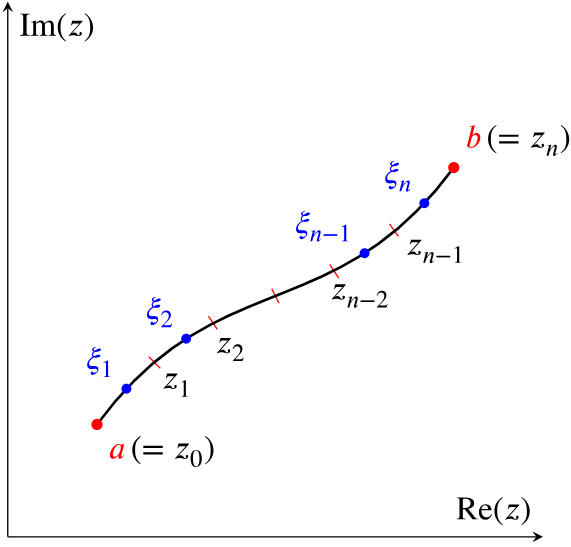
\includegraphics[width=0.4\textwidth]{contour.png}
	\caption{}
	\label{eq:contour}
\end{figure}
We can derive the definition of an integral as the limit of a sum. Let us define a point $z_0 = a$ and $Z_N = b$, and points $z_1$ to $z_{N-1}$ in order on the path. Let us introduce points $t_k$, where $t_k$ is on the path $C$ between $z_{k-1}$ and $z_k$. Let,
\begin{equation}
	\begin{split}
	S_N & = \sum_{k=1}^Nf(t_k)(z_k-z_{k-1}) \\
	& = \sum_{k=1}^Nf(t_k)\Delta z_k.
	\end{split}
\end{equation}
We then define,
\begin{equation}
	\int_C f(z)\dd{z} = \lim_{N \to \infty} S_N
\end{equation}
where all $\Delta z_k \to 0$ as $N \to \infty$. The limit exists if $f(z)$ is continuous on $C$. If we write $\dd{z} = \dd{x} + i\dd{y}$, $\dd{\vb{r}} \equiv \left(\dd{x},\dd{y}\right)$, we have,
\begin{equation}
	\begin{split}
		\int_C f(z)\dd{z} & = \int_Cf(\dd{x} + \dd{y}) \\
		& = \int_C\left[f\dd{x} + (if)\dd{y}\right] \\
		& = \int_C \left(f(z), if(z)\right)\cdot\dd{\vb{r}}.
	\end{split}
\end{equation}
An important contour integral is,
\begin{equation}
	\int_C\frac{1}{z}\dd{z} = 2\pi i \label{eq:2pi}
\end{equation}
where $C$ is a circle of radius $R$.
\subsection{Cauchy's Theorem}
\begin{Theorems}{Cauchy's Theorem}{}
	Suppose $f$ ana. on $C$ and in $S$ enclosed by $C$. Then,
	\begin{equation}
		\oint_C f(z)\dd{z} = 0.
	\end{equation}
\end{Theorems}
\begin{proof}
	Recall Stoke's theorem,
	\begin{align}
		\oint\vb{A}\cdot{\dd{\vb{r}}} &= \int\left(\curl{\vb{A}}\right)\cdot\dd{\vb{S}} \\
		& = {\int\int}_S \left(\pdv{A_y}{x} - \pdv{A_z}{y}\right)\dd{x}\dd{y}
	\end{align}
	for $C$ in $xy$ plane, $\dd{\vb{r}} = (\dd{x},\dd{y}, 0), \dd{\vb{S}} = (0,0,\dd{x}\dd{y})$. On the LHS of Cauchy's theorem,
	\begin{align}
		\oint_C f\dd{z} & = \oint_C f(\dd{x} + i \dd{y}) = \oint_C(\underbrace{f}_{A_x}\dd{x} + \underbrace{(if)}_{A_y}\dd{y}) \\ 
		& = \int\int_S \left(i\pdv{f}{x} - \pdv{f}{y}\right)\dd{x}\dd{y}.\label{eq:A}
	\end{align}
	$f$ is ana.,
	\begin{align}
		\implies & \pdv{f}{x} = \pdv{f}{z}\pdv{z}{x} = \pdv{f}{z} \\
		& \pdv{f}{y} = \pdv{f}{z}\pdv{z}{y} = i\pdv{f}{z}.
	\end{align}
	We then have equation \eqref{eq:A},
	\begin{equation}
		\oint_Cf\dd{z} = \int\int\left(i\pdv{f}{z} - i\pdv{f}{z}\right)\dd{x}\dd{y} = 0.
	\end{equation}
\end{proof}
We can use Cauchy's theorem to show a Corollary which follows naturally: if $f$ ana. between $C_1$ and $C_2$,
\begin{align}
	&\int_{C_1}f\dd{z} - \int_{C_2}f\dd{z} \equiv \oint_{C_1-C_2}f\dd{z} = 0 \\
	\implies \int_{C_1}f\dd{z}=\int_{C_2}f\dd{z}
\end{align}
thus we can deform $C_1$ to $C_2$ if $f$ is ana. in the region between them. 
\\\\
We can furthermore define the image of a function: let $b \equiv z$, i.e., allowing the endpoint to vary,
\begin{equation}
	F(z) = \int_a^zf(s)\dd{s}
\end{equation}
which is well defined if a path is used in the region where f is ana.
\\\\
We can show that differentiation and integration are inverse processes. If we consider the limit as $\Delta z \to 0$,
\begin{equation}
	\frac{F(z+\delta z)-F(z)}{\Delta z} = \frac{1}{\delta Z} \left\{\int_{C_2}f\dd{s} - \int_{C_1}f\dd{s}\right\}
\end{equation}
such that $C_1$ and $C_2$ are paths with the same starting point $a$ but endpoints $F(z)$ and $F(z + \Delta z)$ respectively. We will furthermore consider the path joining $F(z)$ and $F(z+\Delta z)$, $C_3 = C_2 - C_1$. Now, returning to the limit,
\begin{align}
	\frac{1}{\Delta z}\left\{\int_{C_2 - C_1}f\dd s\right\} & = \frac{1}{\Delta z}\int_{C_3}f\dd{s}.
\end{align}
Let us now make a substitution, such that on $C_3$, we take $s(t) = z + t\Delta z$ where $t \in \left[0,1\right]$,
\begin{align}
	&\lim_{\Delta z \to 0}\frac{1}{\Delta z}\int_0^1f(z + \Delta z)\dd{t} \Delta z = \int_0^1f(z)\dd{t} = f(z) \\
	\implies &\dv{F}{z} = f(z).
\end{align}
\subsubsection{Indefinite Integrals}
We can define indefinite integrals by writing,
\begin{equation}
	F(z) = \int^zf(s)\dd{s} = \int f(s) \dd{s}
\end{equation}
given that $f$ is ana everywhere.
\subsubsection{Deformation of Closed Paths}
\begin{figure}[h]
	\centering
	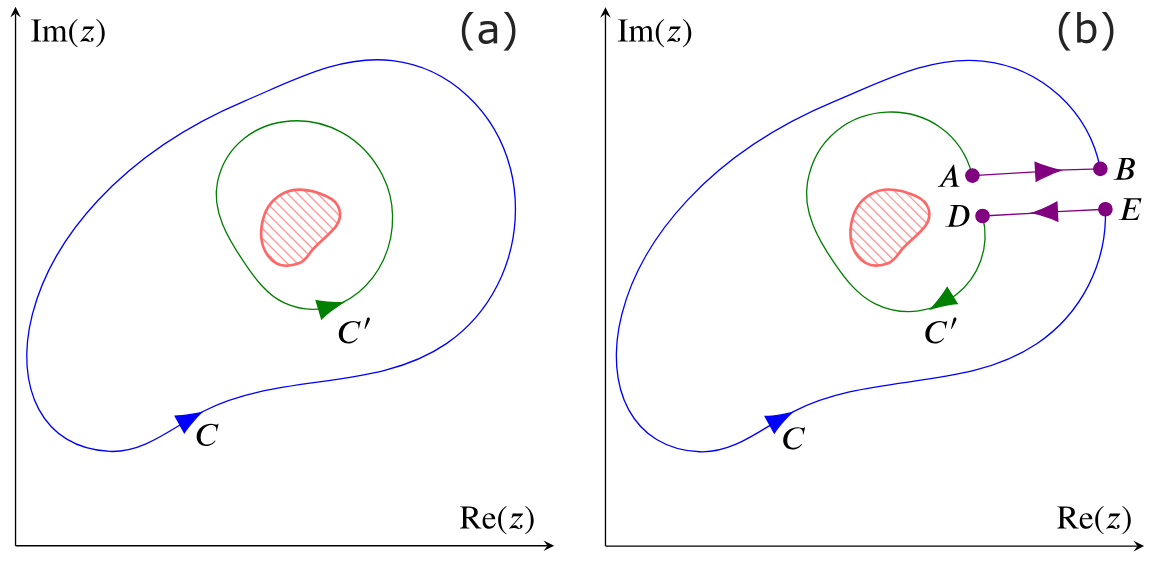
\includegraphics[width=0.6\textwidth]{closed.png}
	\caption{}
	\label{fig:closed}
\end{figure}
\begin{Theorems}{Equivalence of Contours}{}
	Consider figure \ref{fig:closed} (a), where we have two paths $C$ and $C'$ enclosing a non-analytical region. If $f$ is ana between $C$ and $C'$, then,
	\begin{equation}
		\oint_C = \oint_{C'} \neq 0.
	\end{equation}
\end{Theorems}
\begin{proof}
	Now consider \ref{fig:closed} (b), where we have the original paths $C$ and $C'$ but with a break, causing the two paths to become one. The region inside this path is analytic, so must satisfy Cauchy's theorem,
	\begin{equation}
		\int_A^B +\int_B^E + \int_E^D + \int_D^A = 0.
	\end{equation}
	Since $f$ continuous, we can take limits $A \to B$ and $D \to E$,
	\begin{equation}
		\lim_{\substack{A \to D \\ E \to B}} \int_A^B + \int_E^D = 0,
	\end{equation}
	we see that in this limit the straight lines cancel, and the integrals along paths $C$ and $C'$ become closed,
	\begin{align}
		&\int_B^E f\dd{z} \to \oint_C f\dd{z} & \int_D^A f\dd{z} \to -\oint_{C'}f\dd{z} \\
		\implies & \oint_Cf\dd{z} = \oint_{C'} f\dd{z}.
	\end{align}
\end{proof}
\begin{figure}
	\centering
	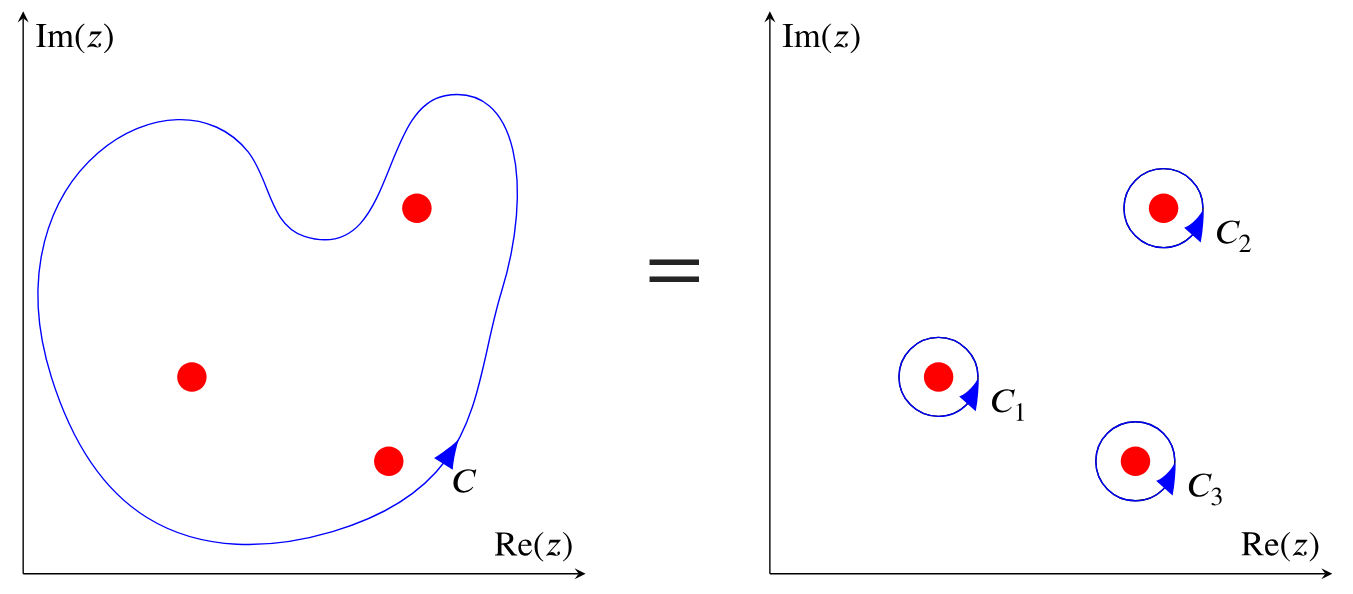
\includegraphics[width=0.6\textwidth]{sing.png}
	\caption{}
	\label{fig:sing}
\end{figure}
We can extend this theorem to multiple singularities. I.e., if we have a single curve $C$ enclosing two singularities, we can decompose the problem into two curves $C_1$ and $C_2$ enclosing each individual singularity, as in figure \ref{fig:sing}. 
\\\\
We have already made use of Cauchy's theorem in the integral \eqref{eq:2pi}. We can generalise this,
\begin{equation}
	\boxed{\oint_C \frac{1}{z-z_0}\dd{z} = \begin{cases}
			2\pi i & C \text{ encircles } z_0\\
			0 & \text{Otherwise}
	\end{cases}}
\end{equation}
\subsection{Cauchy's Integral Formulas}
\begin{Theorems}{}{}
	Suppose $f$ ana on a closed contour $C$ and in the enclosed region. If $z = a$ is a point inside $C$,
	\begin{equation}
		f(a) = \frac{1}{2\pi i }\oint_C \frac{f(z)}{z - a}\dd{z}.
	\end{equation}
\end{Theorems}
\begin{proof}
	Deform $C$ to be a small circle $C'$ centred on $z = a$ with arbitrary radius $\varepsilon$. Then, on $C'$, $z = a + \varepsilon e^{i\theta} \implies \dd{z}=i\varepsilon e^{i\theta}\dd{\theta}$ and,
	\begin{align}
			\oint_{C'} \frac{f(z)}{z-a}\dd{z} &= \int_0^{2\pi}\frac{f(a + \varepsilon e^{i\theta})}{\varepsilon e^{i\theta}}i\varepsilon e^{i\theta} \dd{\theta} \\
			& = i\int_0^{2\pi}f(a + \varepsilon e^{i\theta})\dd{\theta} \\
			& = i \lim_{\varepsilon \to 0} \int_0^{2\pi}f(a + \varepsilon e^{i\theta})\dd{\theta} \\
			& = i \int_0^{2\pi}f(a) \dd{\theta} = 2\pi i f(a).
	\end{align}
\end{proof}
\begin{Theorems}{}{}
	\begin{equation}
		\dv{f(a)}{a} = \frac{1}{2\pi i }\oint_C \frac{f(z)}{(z - a)^2}\dd{z}
	\end{equation}
\end{Theorems}
\begin{proof}
	\begin{align}
		f'(a) & = \lim_{\delta a \to 0}\frac{f(a + \delta a) - f(a)}{\delta a} \\
		&  =\lim_{\delta a \to 0} \frac{1}{\delta a}\frac{1}{2\pi i}\left\{\oint\frac{f(z)}{z - a\delta a}\dd{z} - \oint \frac{f(z)}{z - a}\dd{z}\right\} \\
		& = \lim_{\delta a \to 0} \frac{1}{\delta a}\frac{1}{2\pi i}\oint f(z) \left\{\frac{1}{z - a - \delta a} - \frac{1}{z - a}\right\}\dd{z} \\
		& = \lim_{\delta a \to 0} \frac{1}{\delta a}\frac{1}{2\pi i} \oint f(z) \frac{\Delta a }{(z - a - \delta a)(z - \delta a)}\dd{z} \\
		& = \frac{1}{2\pi i} \oint\frac{f(z)}{(z - a)^2}\dd{z}
	\end{align}
	because $\frac{1}{z-a}$ is continuous.
\end{proof}
We can generalise Theorem 15 by,
\begin{equation}
	\boxed{\dv[n]{f(a)}{a} = \frac{n!}{2\pi i }\oint \frac{f(z)}{(z - a)^{n-1}}\dd{z}}
\end{equation}
\section{Proof of the Fundamental Theorem of Algebra}
\begin{Lemma}{Estimation Lemma for Integrals}{}
	If $\abs{f(z)} \leq m$ on $C$, then $\abs{\int_Cf(z)\dd{z}} \leq mL$ where $L$ is the length of $C$.
\end{Lemma}
\begin{proof}
	\begin{align}
	|S_N| = |\sum_{k=1}^Nf(t_n)\Delta z_k| & \leq \sum_{k=1}^N|f(t_n)||\Delta z_k| \\
	& \leq \sum_{k=1}^Nm|\Delta z_k| = m\sum_{k=1}^N|\Delta z_k|.
	\end{align}
	For $N \to \infty$, $\Delta z_k \to 0$, so,
	\begin{equation}
		|\int_C f(z) \dd{z}| = mL.
	\end{equation}
\end{proof}
\begin{Theorems}{Liouville's Theorem}{}
	If $f$ is bounded on a function $|f(z)| \leq m$, where $m = \text{const.}$, $\forall z$ $\implies f(z) = \text{const.}$.
\end{Theorems}
\begin{proof}
	From Theorem 15, let $C$ be a circle of radius $R$ centred on $z =a$. From the Lemma 1,
	\begin{equation}
		|f'(a)| \leq \frac{1}{2\pi}\frac{M}{R^2}2\pi R = \frac{M}{R}\xrightarrow{R \to \infty} 0.
	\end{equation}
	By definition, $0 \leq f'(a) \leq 0$. This is only consistent if $f'(a) = 0 \implies f(a) = \text{const.}$
\end{proof}
Furthermore, every non-constant ana function becomes arbitrarily big \textit{somewhere}.
\\\\
With these, we can now tackle the fundamental theorem of algebra.
\begin{proof}
	If $P_n(z)$ has no roots, then $\frac{1}{P_n(z)}$ must be analytic everywhere in the complex plane. By Louiville's theorem, $P_n(z)$ is const. This is false, except for $n = 0$. So, $P_n(z)$ must have at least 1 root.
\end{proof}
\section{Taylor Series}
\begin{Theorems}{Taylor's Theorem}{}
If $f(z)$ is ana for $\abs{z -a} < R$, where $R$ is the distance in the complex plane to the closest singularity, then,
\begin{equation}
	f(a) + \frac{(z-a)}{1!}f'(a) + \frac{(z-a)^2}{2!}f''(a) + \cdots 
\end{equation}
converges to $f(z)$.
\end{Theorems}
\begin{proof}
	By Theorem 14, 
	\begin{equation}
		f(z) = \frac{1}{2\pi i }\oint_C \frac{f(s)}{s-z}\dd{s}
	\end{equation}
	with circle $C$ with radius $r < R$ centred on $z = a$. Then,
	\begin{align}
		f(z) & = \frac{1}{2\pi i }\oint_C \frac{f(s)}{(s-a)-(z-a)}\dd{s} \\
		& = \frac{1}{2\pi i}\oint_C \frac{f(s)}{(s-a)\left[1- \underbrace{\frac{z-a}{s-a}}_t\right]}. \label{eq:a}
	\end{align}
	Recall,
	\begin{align}
		\sum_{k=0}^nt_k &= \frac{1-t^{n+1}}{1-t} \\
		\implies \frac{1}{1-t} &= \sum_{k=0}^{n}t^k + \frac{t^{n+1}}{1-t}\label{eq:b}.
	\end{align}
	Combining equations \eqref{eq:a} and \eqref{eq:b},
	\begin{align}
		f(z) &= \sum_{k=0}^{n}\frac{1}{2\pi i }\oint_C\frac{f(s)}{s-a}\left(\frac{z-a}{s-a}\right)^k \dd{s} + \underbrace{\frac{1}{2\pi i}\oint_C \frac{f(s)}{s-a}\left\{\frac{1}{1-\frac{z-a}{s-a}}\left(\frac{z-a}{s-a}\right)^{n+1}\right\}\dd{s}}_{R_n(z,a)} \\
		& = \sum_{k=0}^n(z-a)^k\frac{1}{2\pi i}\oint_C\frac{f(s)}{(s-a)^{k+1}}\dd{s} + R_n(z,a) \\
		& = \sum_{k=0}^n(z-a)^k\frac{f^{(k)}(a)}{k!} + R_n(z,a)
	\end{align}
	by Theorem 15. Using Lemma 1 on $R_n(z,a)$,
	\begin{align}
		|R_n| & =\frac{1}{2\pi}\abs{\oint_Cf(s)\left(\frac{z-a}{s-a}\right)^{(n+1)}\frac{1}{(s-a) - (z-a)}\dd{s}} \\
		\leq \frac{1}{2\pi}m\left(\frac{|z-a|}{r}\right)^{n+1}\frac{1}{r-|z-a|}2\pi r
	\end{align}
	but $\frac{|z-a|}{r} < 1$, so $R_n \xrightarrow{n \to \infty} 0 \implies$ the Taylor series converges to $f(z)$ provided $|z - a| < R$.
\end{proof}
\section{Laurent Series}
The Laurent series generalises the Taylor series to negative powers. 
\begin{Theorems}{Laurent's Theorem}{}
	Consider a function $f(z)$ ana for $R_1 < |z - a| < R_2$. Within the annulus of the circles of radius $R_1$ and $R_2$, $f(z)$ is represented by the Laurent series,
	\begin{equation}
		f(z) = \sum_{n=0}^{\infty}a_n(z-z_0)^n + \sum_{n=1}^{\infty}b_n	\frac{1}{(z-z_0)^n}
	\end{equation}
\end{Theorems}
\begin{proof}
	Let contours $C_1$ and $C_2$ be circles in a region of ana. We will connect $C_1$ and $C_2$ by a bridge $B$ such that the entire contour can be traced by a curve $C$. Using Theorem 14, 
	\begin{equation}
		f(z) = \frac{1}{2\pi i}\oint_C \frac{f(s)}{s - z}\dd{s} \label{eq:23}
	\end{equation}
	we can then also write,
	\begin{equation}
		\oint_C = \int_{C_1} + \int_B + \left(-\int_{C_2}\right) + (-\int_B) = \int_{C_1} - \int_{C_2},
	\end{equation}
	thus, we write equation \eqref{eq:23},
	\begin{equation}
		f(z) = \frac{1}{2\pi i}\oint_{C_1}\frac{f(s)}{s - z}\dd{s} -\frac{1}{2\pi i}\oint_{C_2}\frac{f(s)}{s-z}\dd{s}.
	\end{equation}
	We will now proceed as with the proof for Taylor's series, however we will ignore the remainder terms as we already know they converge to 0. For the region where $|s - a| > |z - a|$,
	\begin{equation}
		\begin{split}
			\frac{1}{s - z} &= \frac{1}{(s - a)-(z-a)} = \frac{1}{s - a}\left(1 - \frac{z -a}{s-a}\right)^{-1} \\
			& = \frac{1}{s-z}\sum_{k=0}^{\infty}\left(\frac{z-a}{s-a}\right)^k + \cdots
		\end{split}
	\end{equation}
	We then write,
	\begin{equation}
		\begin{split}
		\frac{1}{2\pi i }\oint_{C_1} \frac{f(s)}{s-z} &= \sum_{k=0}^{\infty}\frac{1}{2\pi i}\oint_{C_1}\frac{f(s)(z-a)^k}{(s-a)^{k+1}}\dd{s} \\
		& = \sum_{k=0}^{\infty} a_k(z -a)^k
		\end{split}
	\end{equation}
	where,
	\begin{equation}
		a_k = \frac{1}{2\pi i }\oint_{C_1} \frac{f(s)}{(s-a)^{n+1}}\dd{s}.
	\end{equation}
	Repeating this for the case $|s - a| < |z - a|$,
	\begin{equation}
		\begin{split}
			\frac{1}{s-a} = \frac{1}{(s-a)-(z-a)} & = -\frac{1}{z-a}\left(1-\frac{s-a}{z-a}\right)^{-1} \\
			& = -\frac{1}{z-a}\sum_{k=0}^{\infty}\left(\frac{s-a}{z-a}\right)^{k}.
		\end{split}
	\end{equation}
	We then write,
	\begin{equation}
		-\frac{1}{2\pi i }\oint_{C_2} \frac{f(s)}{s-z} = \sum_{k=1}^{\infty}\frac{a_{-k}}{(z-a)^k}
	\end{equation}
	where
	\begin{equation}
		a_{-k} = \frac{1}{2\pi i }\oint_{C_2}f(s) (s-a)^{k-1}\dd{s}.
	\end{equation}
	As $f$ ana between $C_1$ and $C_2$, we can replace $C_1$ and $C_2$ with any contour $C$ lying in the annulus of convergence.
\end{proof}
The part with positive powers is known as the \textit{analytic} part of the function, and the part with negative powers is known as the \textit{principal} part.
\subsection{Residue Theorem}
A residue is the first non-zero term in the principal part of the Laurent series expanded about a singular point $z = z_0$. If a function has a Laurent series valid within $0 < |z - z_0| < R$, then the integral around a contour $C$ within those bounds is given by,
\begin{equation}
	\oint_C f(z) \dd{z} 2\pi i a_{-1}.
\end{equation}
The residue $b_1$ is the residue of $f(z)$ at $z = z_0$, often denoted $\text{res}(z_0)$. 
\begin{Theorems}{Residue Theorem}{}
	If a curve $C$ encloses $p$ poles $z_i$, $i=1,\ldots, p$ of $f(z)$, the contour integral around $C$ is,
	\begin{equation}
		\oint_C f(z) \dd{z} =2\pi i\sum_{j=1}^p\text{res}(z_j).
	\end{equation}
\end{Theorems}
\subsubsection{Methods of finding residues}
\begin{enumerate}
	\item Suppose $f(z)$ has a \textit{simple} pole at $z = a$ $\implies$ $g(z) = (z-a)f(z)$ is ana at $z=a$ so a Taylor series,
	\begin{align}
		& g(z) =  g(a) + (z-a)g'(a) + \mathcal{O}\left((z-a)^2\right) \\
		\implies & f(z) = \frac{g(a)}{z-a} + g'(a) + \mathcal{O}(z-a) \\
		\implies & \text{res}(a) = g(a) = \lim_{z \to a}\left\{(z-a)f(z)\right\}
	\end{align}
	\begin{enumerate}
		\item \textit{Popular Exam Question:} $f(z) = \frac{1}{\sin z}$ has simple poles at $z = n\pi, n \in \mathbb{Z}$.
		\\\\
		To do this, we set $z = n\pi + \varepsilon$ where $\varepsilon << 1$, and solve,
		\begin{equation}
			\text{res}(n\pi) = \lim_{z \to n\pi}\left\{(z-n\pi)\frac{1}{\sin(z)}\right\} = \lim_{\varepsilon\to0}\left\{\frac{\varepsilon}{\sin(n\pi + \varepsilon)}\right\}.
		\end{equation}
	\end{enumerate}
	\item For $f(z) = \frac{g(z)}{h(z)}$ where $g,h$ ana at $z=a$, $g(a) \neq 0$ but $h(a) = 0$, $h'(a) \neq 0 \implies h(z) = (z-a)h'(a) + \mathcal{O}\left((z-a)^3\right)$ thus,
	\begin{equation}
		\begin{split}
			\text{res}(a) & = \lim_{z \to a}\left\{(z-a)\frac{g(z)}{(z-a)h'(a) + \mathcal{O}\left((z-a)^2\right)}\right\} \\
			& = \lim_{z \to a}\left\{\frac{g(z)}{h'(a) + \mathcal{O}(z-a)}\right\} = \frac{g(a)}{h'(a)}
		\end{split}
	\end{equation}
	\item Suppose $f$ has a pole of order $p$ at $z = a$ $\implies g(z) = (z-a)^pf(z)$ is ana at $z=a$ and has a Taylor expansion,
	\begin{align}
		& g(z) = g(a) + \frac{z-a}{1!}g'(a) + \cdots + \frac{(z-a)^{(p-1)}}{(p-1)!}g^{(p-1)}(a) + \cdots \\
		\implies & f(z) = \frac{g(a)}{(z-a)^p} + \cdots + \frac{1}{z-a}\left\{\frac{g^{(p-1)}(a)}{(p-1)!}\right\} + \cdots
	\end{align}
	thus, generally,
	\begin{equation}
		\boxed{\text{res}(a) = \frac{g^{(p-a)(a)}}{(p-1)!} = \frac{1}{(p-1)!}\lim_{z\to a}\left\{\dv[p-1]{z}\left[(z-a)^pf(z)\right]\right\}}
	\end{equation}
\end{enumerate}
\section{Complex Methods of Real Integrals}

\end{document}
 